\documentclass[11pt]{scrartcl}
\usepackage[sexy]{evan}
\usepackage{graphicx}

\newcommand{\N}{\mathbb{N}}
\newcommand{\Z}{\mathbb{Z}}
\newcommand{\F}{\mathbb{F}}
\newcommand{\Q}{\mathbb{Q}}
\newcommand{\R}{\mathbb{R}}
\newcommand{\C}{\mathbb C}


\newcommand{\Vu}{\mathbf{u}}
\newcommand{\Vv}{\mathbf{v}}
\newcommand{\Vw}{\mathbf{w}}
\newcommand{\Vx}{\mathbf{x}}
\newcommand{\Ve}{\mathbf{e}}
\newcommand{\Vc}{\mathbf{c}}
\newcommand{\Vb}{\mathbf{b}}



\newcommand{\Va}{\mathbf{a}}

\newcommand{\Vhx}{\mathbf{\hat{x}}}

\newcommand{\Vy}{\mathbf{y}}
\newcommand{\Vz}{\mathbf{z}}
\newcommand{\Vo}{\mathbf{0}}

%From Topology
\newcommand{\cT}{\mathcal{T}}
\newcommand{\cB}{\mathcal{B}}
\newcommand{\cC}{\mathcal{C}}

\usepackage{answers}
\Newassociation{hint}{hintitem}{all-hints}
\renewcommand{\solutionextension}{out}
\renewenvironment{hintitem}[1]{\item[\bfseries #1.]}{}
\declaretheorem[style=thmbluebox,name={Theorem}]{thm}

\begin{document}
\title{CS 182}
\author{Vishal Raman}
\thispagestyle{empty}
$ $
\vfill
\begin{center}

\centerline{\huge \textbf{CS 182 Lecture Notes, Spring 2022}}
\centerline{\Large \textbf{Deep Learning} } 
\centerline{Professor: Marvin Zhang}
\centerline{Vishal Raman}
\end{center}
\vfill
$ $
\newpage
\thispagestyle{empty}
\tableofcontents
\newpage
%\maketitle
\section{02/28/2022 - Recurrent Neural Networks}
\subsection{Problem Setup}
We consider settings in which the features $\textbf{x}$ represent \textit{sequential data} which may be \textbf{variable length}. Some examples include
\begin{itemize}
\item Text of different lengths
\item Audio recordings/waves
\item Video recordings
\end{itemize} 
The labels could be scalars $y$(sentiment analysis, identification), or they could be sequences $\textbf{y}$(translation, transcription, captioning).  There could also be 
no label at all!  This is true in unsupervised learning/generating modeling.

Some models we use include:
\begin{itemize}
\item Markov/n-gram models, hidden Markov models(HMMs)
\item Embedding/clustering-based methods
\item Convolutions("temporal" convolutions which could be a 1-d convolution of a sequence, or a 3-d convolution over a video).
\item Recurrent Neural Networks(RNNs)
\item Long short-term memory(LSTM)
\item Gated Recurrent Units(GRUs)
\item Transformers
\end{itemize}

\subsection{Dealing with Variable Length Inputs}
Before, when dealing with images, we could reasonably assume fixed size inputs.  However, with sequential data, it can be assumed that the input lengths will almost always vary. 
\begin{center}
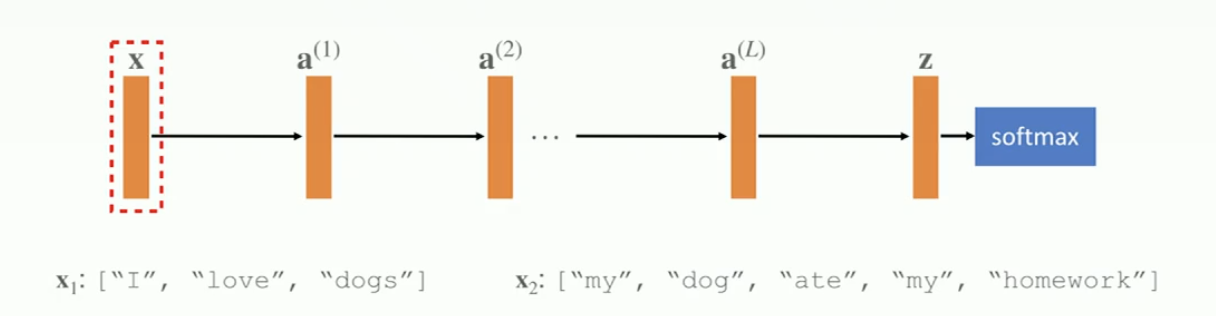
\includegraphics[scale=0.5]{images/var_length.png}
\end{center}

To deal with this, we feed one piece of input called a \textbf{token} per layer. 
\begin{center}
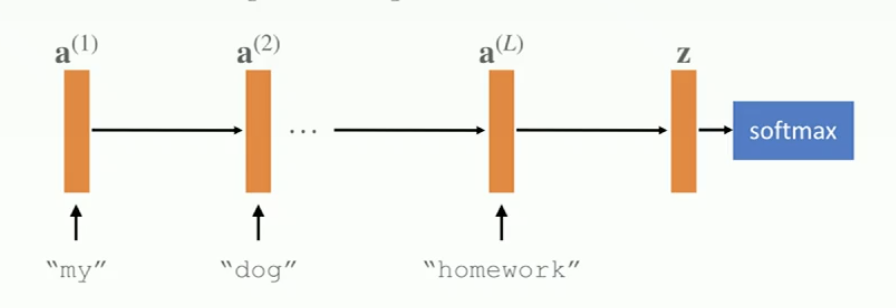
\includegraphics[scale=0.5]{images/token.png}
\end{center}
Now, the input to layer $\ell + 1$ is $[a^{(\ell)}; x[\ell] ]$.

The issues with this approach are the following:
\begin{itemize}
\item We need as many layers as the max number of tokens.  For very large inputs, we would have extremely deep networks which are difficult to train.
\item We have a different $W^{(\ell)}$ and $b^{(\ell)}$ for each layer, which is a massive number of items to optimize.  
\item The later layers get trained very rarely, so it's hard to generalize to longer sequences at test time.  
\item Another issue is that $a^{(1)}$ is missing the previous layer output. 
\end{itemize}
\subsection{Recurrent Neural Networks}
To solve some of these issues, we use \textbf{weight sharing}: use the same parameters in every layer.
$$\text{Before: } a^{(l + 1)} = \sigma(W^{(l + 1)}[a^{(l)}; x[l]] + b^{(l + 1)})$$
$$\text{Now: } a^{(l + 1)} = \sigma(W[a^{(l)}; x[l]] + b)$$

\begin{remark} In backpropagation, $W$ and $b$ get a gradient signal from every single time they are applied in the network, and we sum them to get the final gradient for $W$ and $b$.
\end{remark}

To address the problem with $a^{(1)}$, initialize some $a^{(0)}$ independently from the input $x$ and feed it into $a^{(1)}.$

Putting these two ideas together gives us the Recurrent Neural Network(RNN).

\begin{remark} The values $x[l]$ are encoded from some word2vec algorithm and the end vector is the same length for each word.
\end{remark}
\
The above applies for a sequence input, single output.  If we wanted sequence input, sequence output, we could output a scalar at each layer to get a sequence output.
\begin{center}
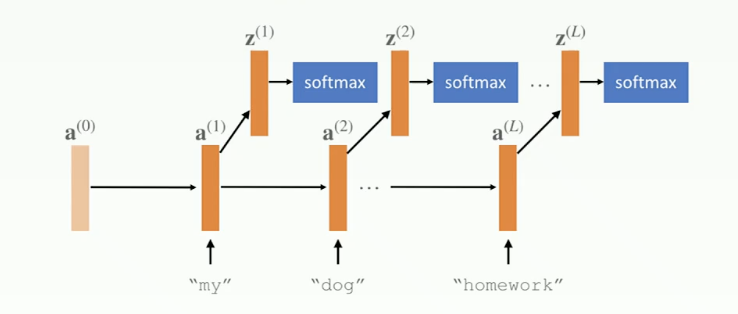
\includegraphics[scale=0.8]{images/seqout.png}
\end{center}

In general, different applications give rise to different ways we use RNNs.

\begin{center}
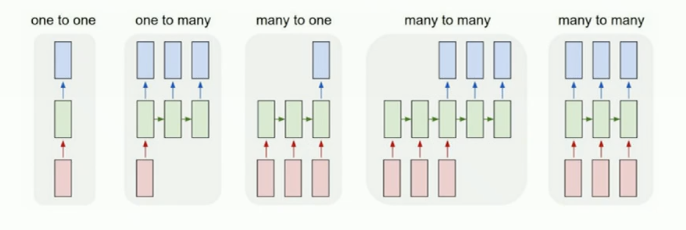
\includegraphics[scale=0.8]{images/atob.png}
\end{center}
\begin{itemize}
\item One-to-one is not an RNN.  It is like the ConvNet or Fully-Connected Net we have worked with.
\item For translation, we might do something like the 4th diagram, since we need to see the whole sentence before we can translate.
\item Image Captioning is single input, sequence output.
\item Sentiment Analysis is many to one, sequence input single output.
\item Text generation would be many to many like the last diagram.  
\item The many-to-many can have many different styles depending on the application.
\end{itemize}

\subsection{Generating Outputs from RNNs}
Generating a sequential output is done in an \textbf{autoregressive} manner: condition the model on what you have seen before to generate the next thing. 
\begin{center}
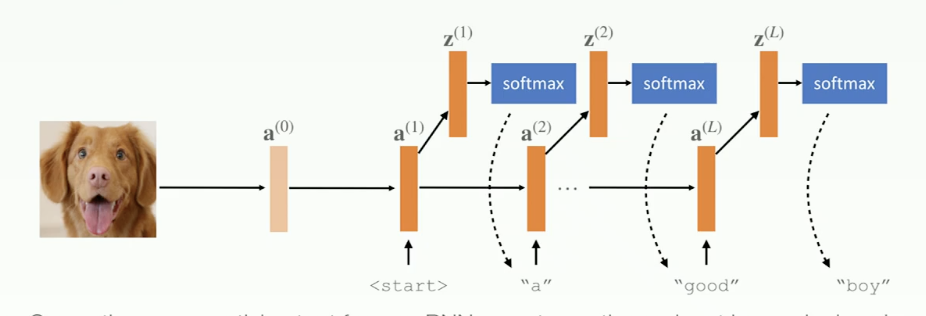
\includegraphics[scale=0.8]{images/autoreg.png}
\end{center}
\begin{remark} In the above, we assume that the RNN is already trained, and then we use it to generate text using the above scheme. 
\end{remark}

\subsection{Vanishing/Exploding Gradients}
What is the gradient of the final loss with respect to $W/b$?
\begin{center}
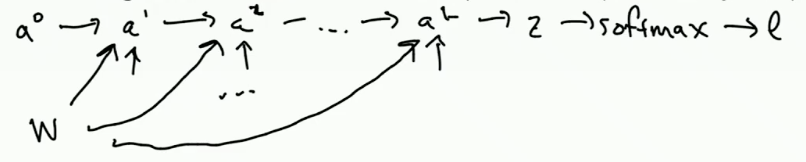
\includegraphics[scale=0.8]{images/grad.png}
\end{center}

We have 
$$\frac{d\ell}{dW} = \sum_{k=1}
^L \frac{d\ell}{da^k} \frac{da^k}{dW},$$
$$\frac{d\ell}{da^{1}} = \frac{d\ell}{da^L} \frac{da^L}{da^{L-1}} \dots \frac{da^2}{da^1},$$
so it is very easy for gradients to vanish or explode.

We can deal with this as follows:
\begin{itemize}
\item For exploding gradients, we can just \textbf{clip} the gradients - divide by the magnitude of the large gradients to make them smaller.
\item Vanishing gradients seem to require clever architecture choices: one idea we can use to address this is a \textbf{skip connection}!  
\item One architecture that does this is the \textbf{LSTM}: it is much older than skip-connections but employs the same basic principle that allow better gradient flow by making smarter connection choices. 
\end{itemize}
\pagebreak
\section{02/28/2022 - Long Short-Term Memory(LSTM)}
\begin{center}
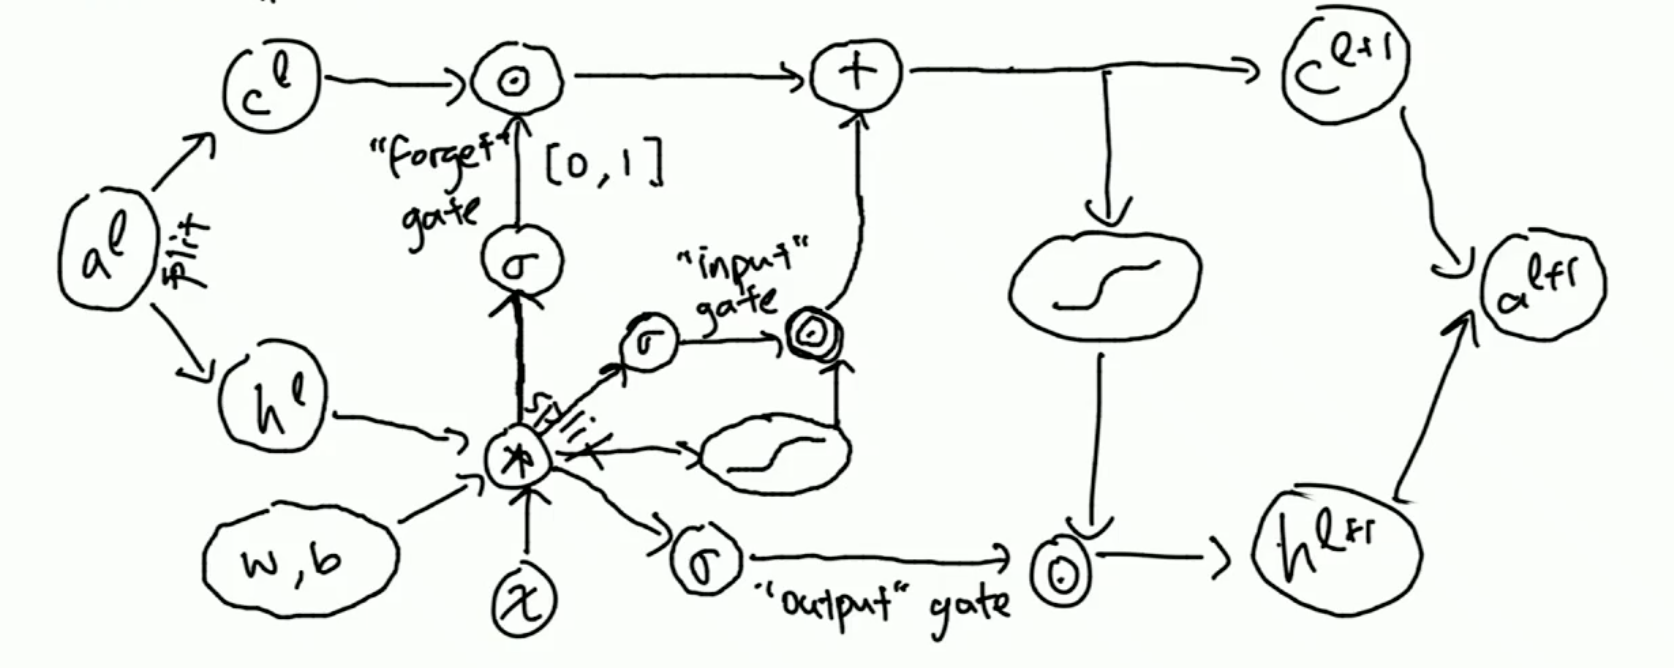
\includegraphics[scale=0.5]{images/lstm.png}
\end{center}

\begin{enumerate}
\item Start with a state $a^{\ell}$ and split into two states, $c^\ell$ the cell state, and $h^{\ell}$ the hidden state.  We have $d_{c} = d_h$, and $d_a = d_c + d_h$, since we exactly split $a$ into two parts. 
\begin{itemize}
\item $c^\ell$ is the part that acts like a skip so we have better gradient flow with long sequences.  
\item $h^\ell$ deals with the nonlinearities which we need for expressivity. 
\end{itemize}
\item For the cell state $c^\ell$, we element-wise multiply by scalars $f^\ell$ in $[0, 1]$(we can do this by passing some number into the sigmoid $\sigma$).  This is the \textbf{forget gate} - when the scalar is close to $0$, we forget these dimensions, and when the scalars are close to $1$, we retain the information and gradient flow.  Then, we add a bias $i^\ell$, which is called the \textbf{input} to the cell state.  This gives us $c^{\ell + 1}$.  Overall, we have 
$$c^{\ell + 1} = c^{\ell} \odot f^{\ell} + i^\ell.$$
\item For the hidden state $h^\ell$, we use an affine transformation using parameters $W, b$ and the input $x$.  This is split into $4$ equal parts each with the same dimension as $h$:
\begin{itemize}
\item The first piece determines $f^\ell$, the element sent into the \textbf{forget gate}.
\item The next piece is sent to a nonlinearity(doesn't matter which one) and a piece sent to the sigmoid which is elementwise-multiplied to the nonlinearity output.  This is called the \textbf{input gate}.
\item The last piece is sent to a sigmoid to be used for the output gate.
\end{itemize}
\item We also take $c^{l+1}$ and use a nonlinearity(doesn't matter which one) and element-wise multiplied by the component from the output gate to determine $h^{l+1}$.
\end{enumerate}

\begin{remark} Some elements are important but others are pretty arbitrary.  For example, the GRU is very similar but it doesn't have an output gate.  However, it still performs pretty well.
\end{remark}

\subsection{Bidirectional RNN Models}
Often, it can be useful to incorporate information from "the future".  For example, when doing speech transcription, if we take an audio waveform and transcribe that into words, it might be useful to see the piece corresponding to the end of the word before the beginning of the word.  Similarly, when doing contextual word representations, a word might have different interpretations based on the words around it("my back hurts", "my back door is open").

To do this, one option is to learn two RNNs!  One processes the sequence in the forward direction and one does the reverse.  But they are learned jointly to produce a single prediction/representation.

For a while, bidirectional LSTMs were the best model for learning language representations that can be fine tuned for a variety of downstream tasks(ELMo-embeddings from language models).  But now we have transformers(BERT).

\pagebreak
\section{3/7/2022 - Transformers}
\subsection{Setup}
We start with features $x$, which could be sequential data of variable length:
\begin{itemize}
\item Text
\item Audio Waves
\item Videos
\end{itemize}

We have labels $y$ given by 
\begin{itemize}
\item Sentiment analysis or translation
\item audio transcription or speaker identification
\item activity identification or video captioning
\item No label! Unsupervised learning or generative modeling
\end{itemize}

We will use transformers to deal with these.
\subsection{Why Transformers}
These have been massively influential in the past 4-5 years.  They have been outcompeting other deep architectures, such as RNNs in language modeling and ConvNets in vision tasks.
\begin{remark} This is pretty insane since we have such strong inductive biases for ConvNets.
\end{remark}
There are other modern models using \textit{attention}, while they are not really transformers.

They are the backbone of BERT and GPT and they perform language tasks at a level which we didn't think was possible a few years ago. For this reason, people dub these as "foundation models".
\subsection{Attention}
Originally formulated for tasks with sequential outputs. 
\begin{itemize}
\item Translating between languages, captioning an image
\item The features may not be sequential: for example, we could have an image, pass it through a model, and output a sequential caption vector.
\end{itemize}


\begin{center}
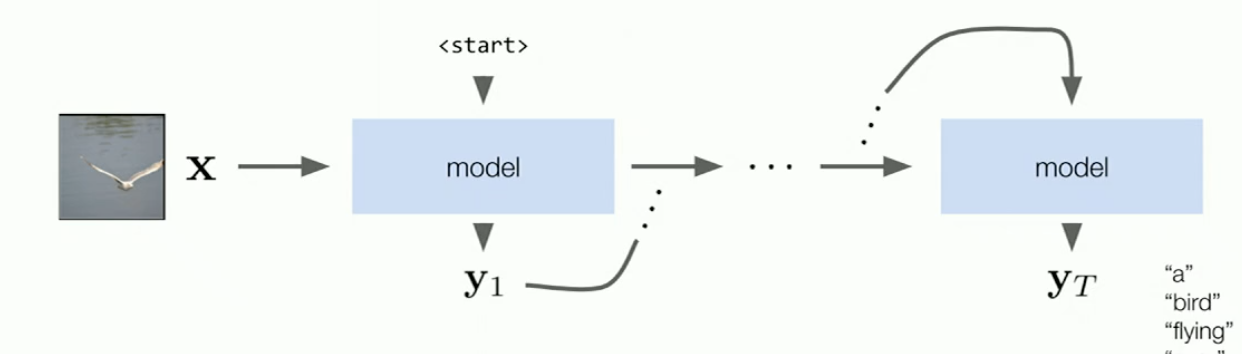
\includegraphics[scale=0.5]{images/attention1.png}
\end{center}
We will generate the output one step at a time. However, we need to know what we have generated so far.  We could handle this via \textit{autoregressive generation} from an RNN, where we feed model output into the next input until we have generated an entire sequence of tokens. 

Now, we motivate attention.  For example with the caption, "A bird flying over a body of water .", we maybe want the model to focus on the parts of the image focusing on the recently generated token:
\begin{center}
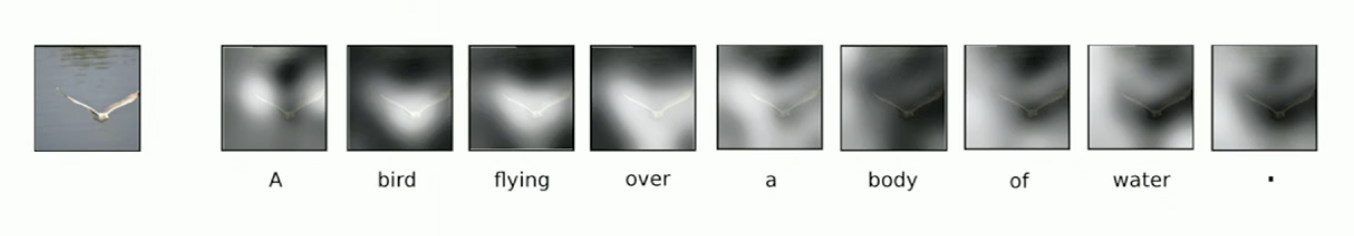
\includegraphics[scale=0.5]{images/intuition.png}
\end{center}

\subsubsection{What to attend over?}
\begin{itemize}
\item If the features are words, we can attend over them directly.
\item If the features are pixels, we can pass the image through the top layers of a ConvNet(usually pretrained on image net).  This gives us an intermediate representation of an image, and these low dimensional representations give some understanding of high level features.  
\end{itemize}
\begin{remark} Why did they not train the layers end-to-end?  Possibly for optimization reasons, compute difficulties?  But if this was done today, would probably be end-to-end.  
\end{remark}
\subsubsection{Details of Attention}
After passing the image through the ConvNet, we have $L$ context vectors from hopefully corresponding to different semantic elements of the image.  Then, we pass these into the model to generate an output token.  Then, we can pass this output into the next model in an auto-regressive fashion.  
\begin{center}
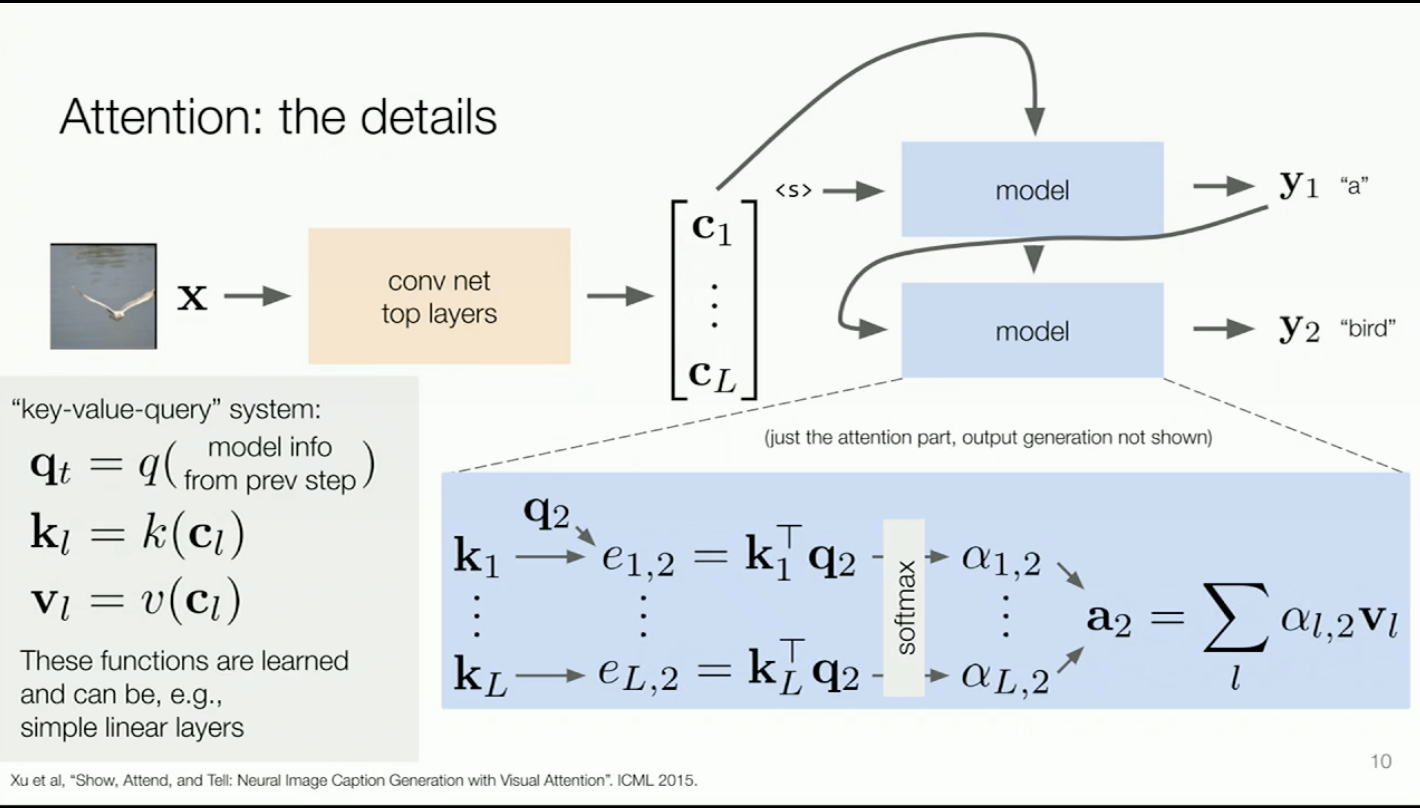
\includegraphics[scale=0.5]{images/details.png}
\end{center}
\begin{remark} Note that everything here is differentiable, so we can backprop and learn $k, q, v$ through auto-diff.  
\end{remark}
\subsubsection{Self-Attention}
The goal of self-attention is to handle sequential features as the input.  We can think of it as a layer that processes the entire sequence which produces intermediate activations $a_1 \to a_t$.  Now, we have 
$$q_t = q(x_t), k_t = k(x_t), v_t = v(x_t).$$
\begin{center}
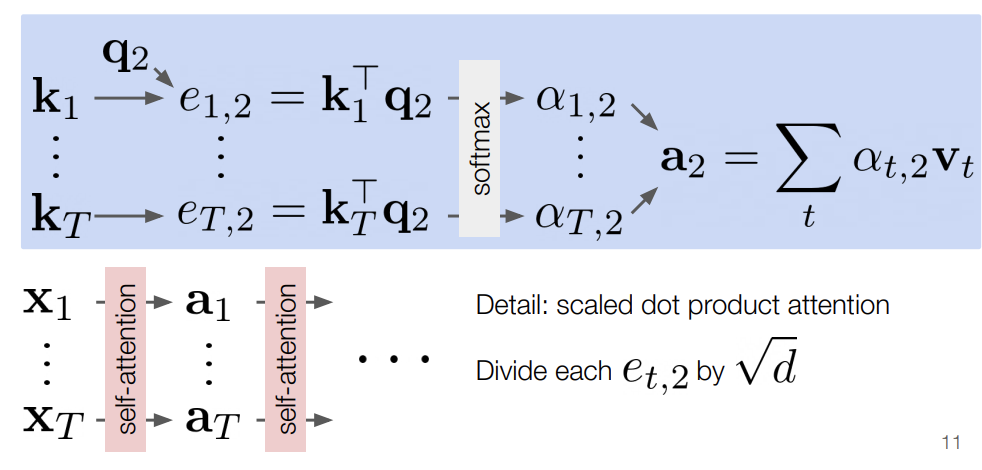
\includegraphics[scale=0.5]{images/self-atten.png}
\end{center}
\begin{remark} One problem that we have is that self-attention is completely linear function of the inputs.  So we need to interweave these with nonlinearities.  
\end{remark}
\begin{remark} We also have scaled dot product attention, where we divide each $e_{t, 2}$ by $\sqrt{d}$.  This is similar to weight-initialization.
\end{remark}
\begin{remark} It seems like the ordering of the elements do not matter in the case of self-attention.  This is true and is handled by transformers.
\end{remark}

\subsection{Transformers}
\subsubsection{Transformer Encoder}
We start with a vector $X \to Z$, through a transformer encoder.  
\begin{center}
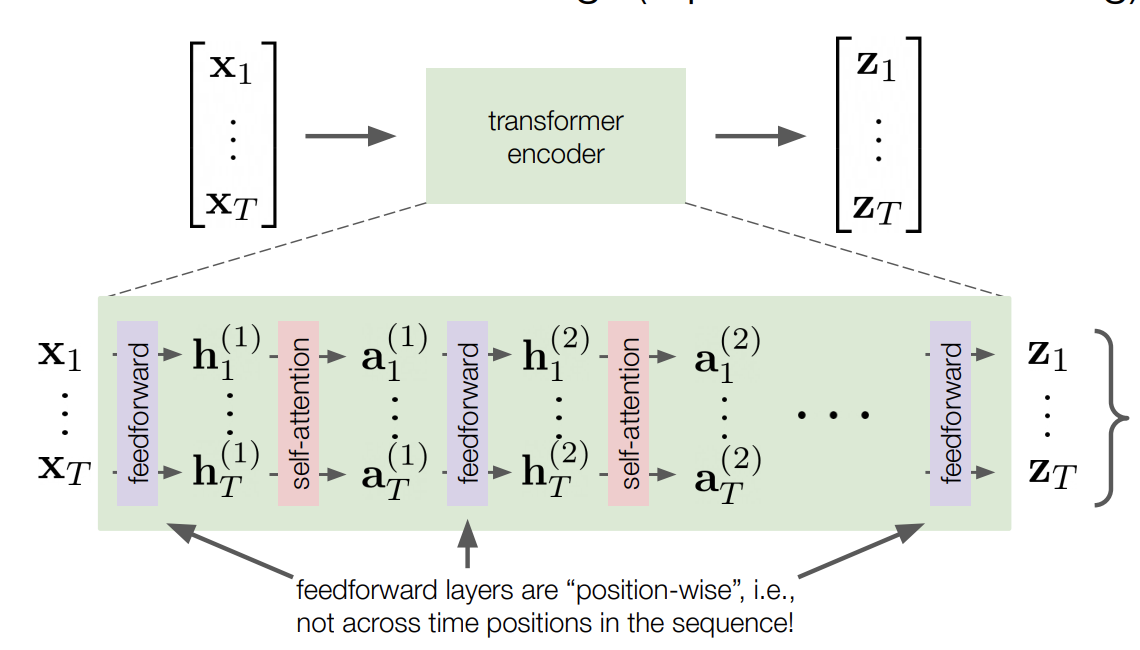
\includegraphics[scale=0.5]{images/encoder.png}
\end{center}
\begin{remark} Note that for the feedforward layers, $h_i^{(1)}$ depends only on $x_i$ and the same is true for the later layers.  
\end{remark}

\subsubsection{Positional Encoding}
After the feedforward layer, a positional encoding is added to each $h_t^{(1)}$.  This is some information about what time-step each input corresponds to.  Without this, the model cannot distinguish between different permutations of the input sequence.  One choice is to add the following vector to $h_t$:
\begin{center}
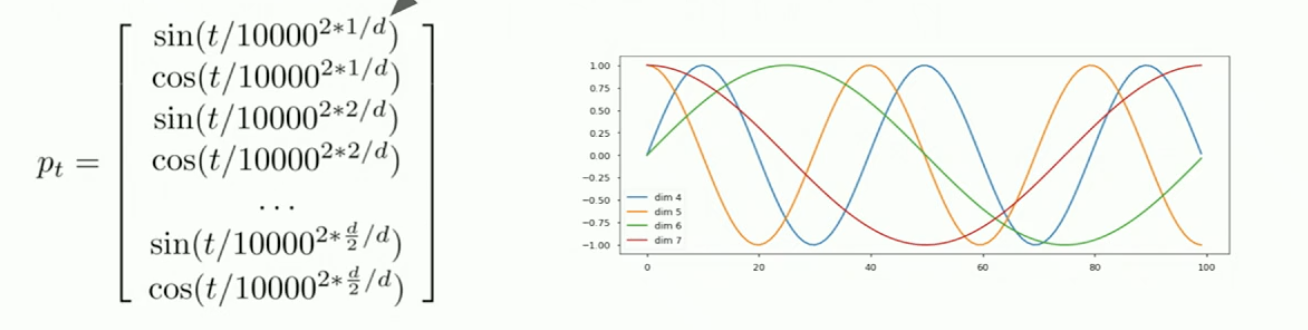
\includegraphics[scale=0.5]{images/position.png}
\end{center}

Are there alternatives to this?  What if we just concatenated the time step after the first feed-forward layer?  This appears worse because we care more about the relative positioning:
\begin{center}
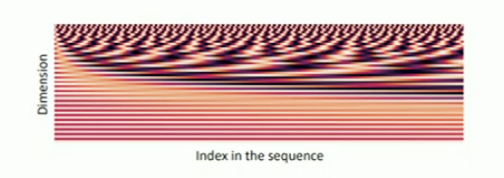
\includegraphics[scale=1.5]{images/relativepos.png}
\end{center}
What if we learned the positional encodings?  This is used sometimes and sometimes better due to expressivity.  However, this has downsides: can't generalize to longer sequences, etc. 
\subsubsection{Multi-Head Attention}
Starting with self attention, we have a mechinism going from $\mathbb{x} \to \mathbb{a}$, where $\mathbb{a}_2 = \sum_t \alpha_{t, 2} \mathbb{v}_t$.  This works well if we have one particular key that we should pay attention to.  But what if we have multiple features that we want to pay attention to?  We can do this by having "multiple heads", which are independent attention blocks that pay attention to different values.  
\begin{center}
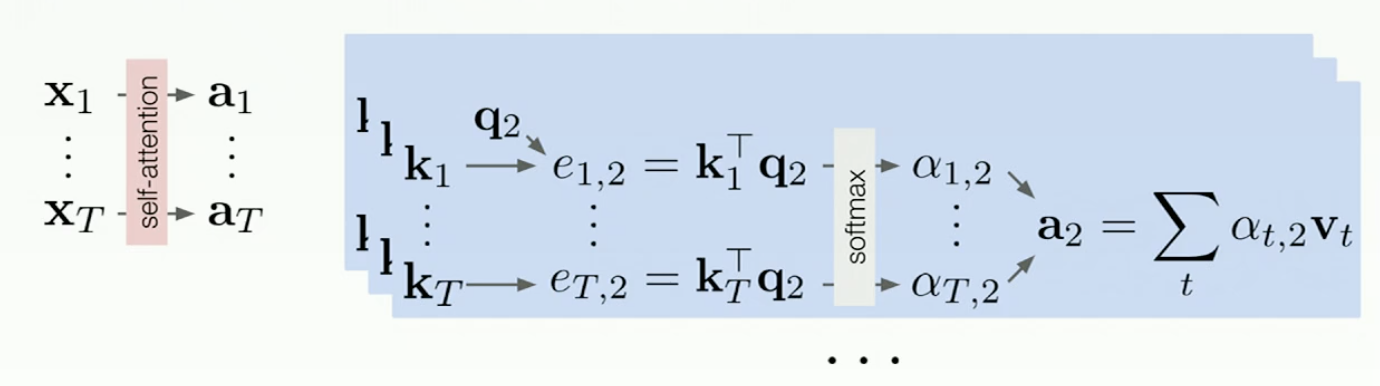
\includegraphics[scale=0.5]{images/multihead.png}
\end{center}
\begin{remark} Note that each of the key, query, and value functions for each head have their own learned parameters.
\end{remark}
\begin{remark} The final $a_2$ and every $a_t$ is given by concatenating the outputs from each head and potentially feeding this through another linear layer.  
\end{remark}
\begin{remark} In order to not make this not scale linearly in complexity with the number of heads, we scale the dimension down proportionally to the number of heads, e.g.,  if 512 dimensions for 1 head, then 64 dimensions for 8 heads.    
\end{remark}
The final picture for the encoder is given by 
\begin{center}
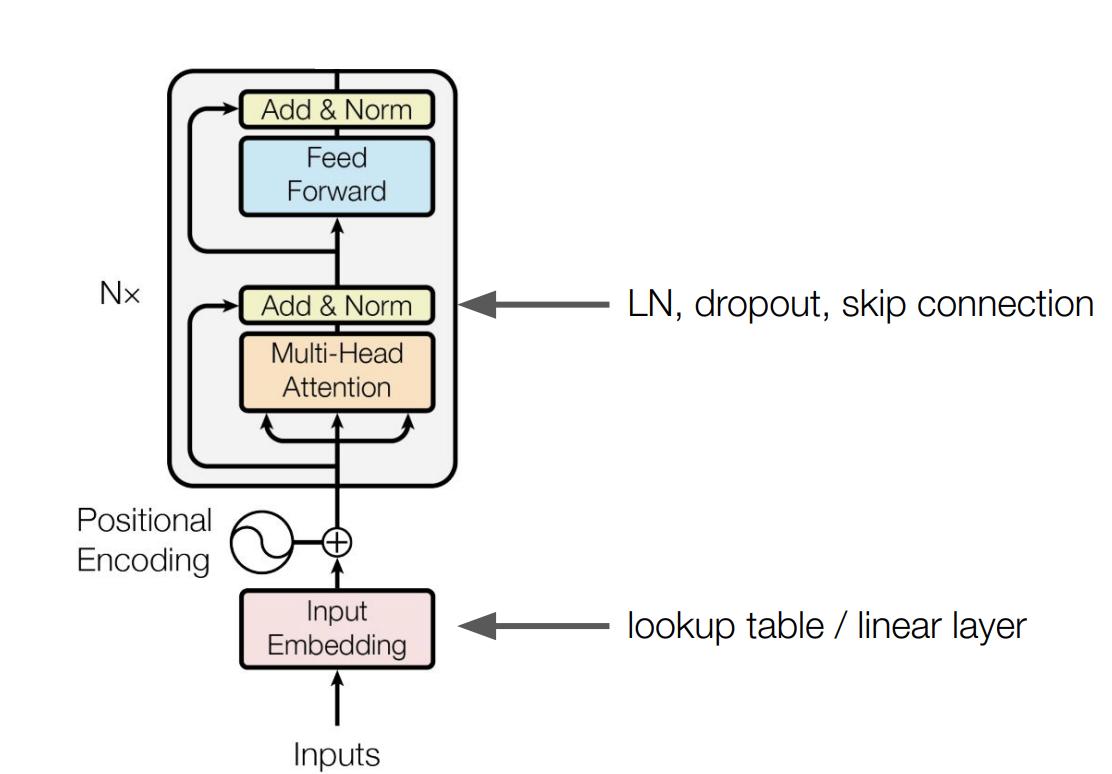
\includegraphics[scale=0.5]{images/encoder-final.png}
\end{center}

\subsubsection{Transformer Decoder}
As before, we feed the outputs of the decoder into the Transformer decoder as input.  However, at training time, we feed ground truth sentences in the decoder.  

\begin{center}
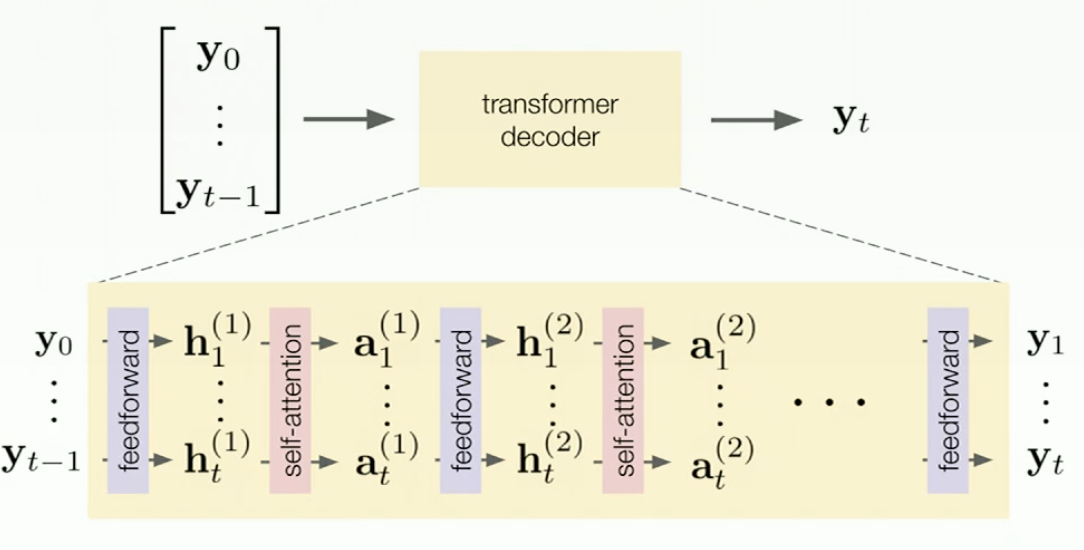
\includegraphics[scale=0.5]{images/decoder.png}
\end{center}

\subsubsection{Masked Attention}
During training, we are passing entire sequences instead of passing in partial sequences since this is more computationally efficient.  However, the model cannot be looking at the future to generate earlier elements from later ones.  To do this, we "mask" the keys and values corresponding to future timesteps.  

\begin{center}
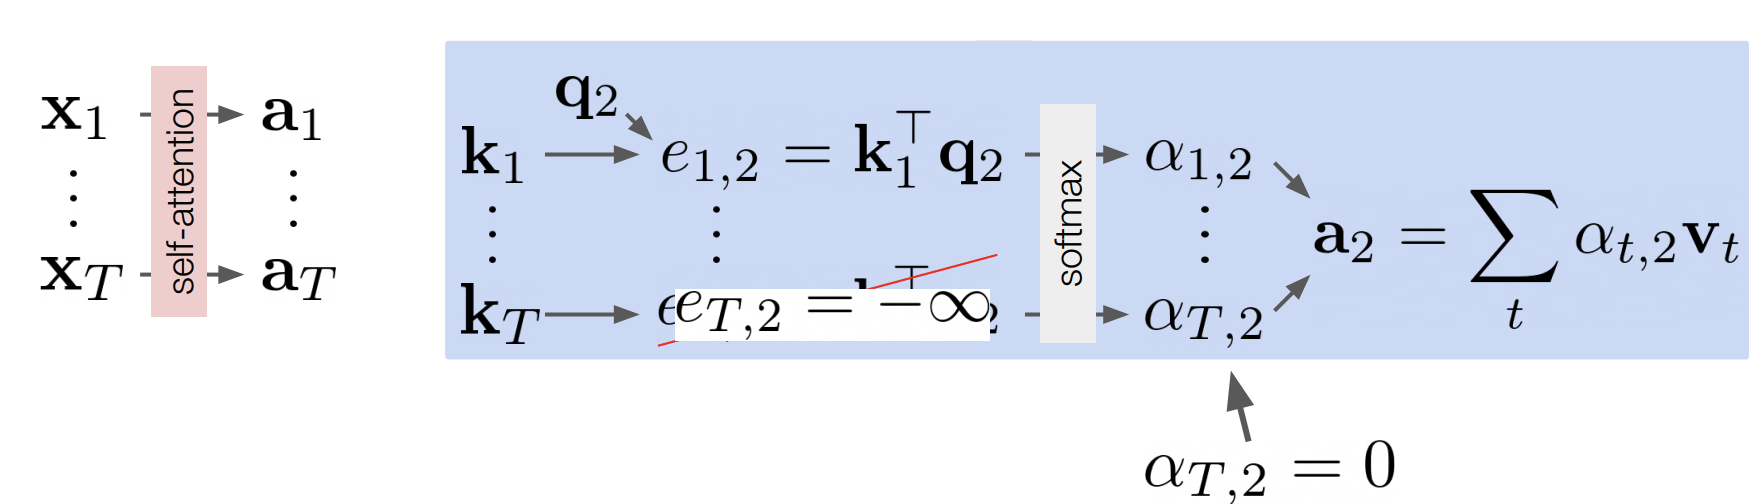
\includegraphics[scale=0.5]{images/masked.png}
\end{center}

\pagebreak
\section{03/09/2022 - Transformer Models}
The original transformer is a sequence-to-sequence model for translation.  These typically follow an encoder-decoder architecture and the transformer does well at handling these tasks. We will go into sequence-to-sequence models more in the future.
\subsection{Encoder: BERT}
During training, input tokens(words) are randomly masked with $p = 0.15$.  The model must predict these tokens before they were masked.  The hypothesis is that it allows BERT to learn word level representations.  

\begin{center}
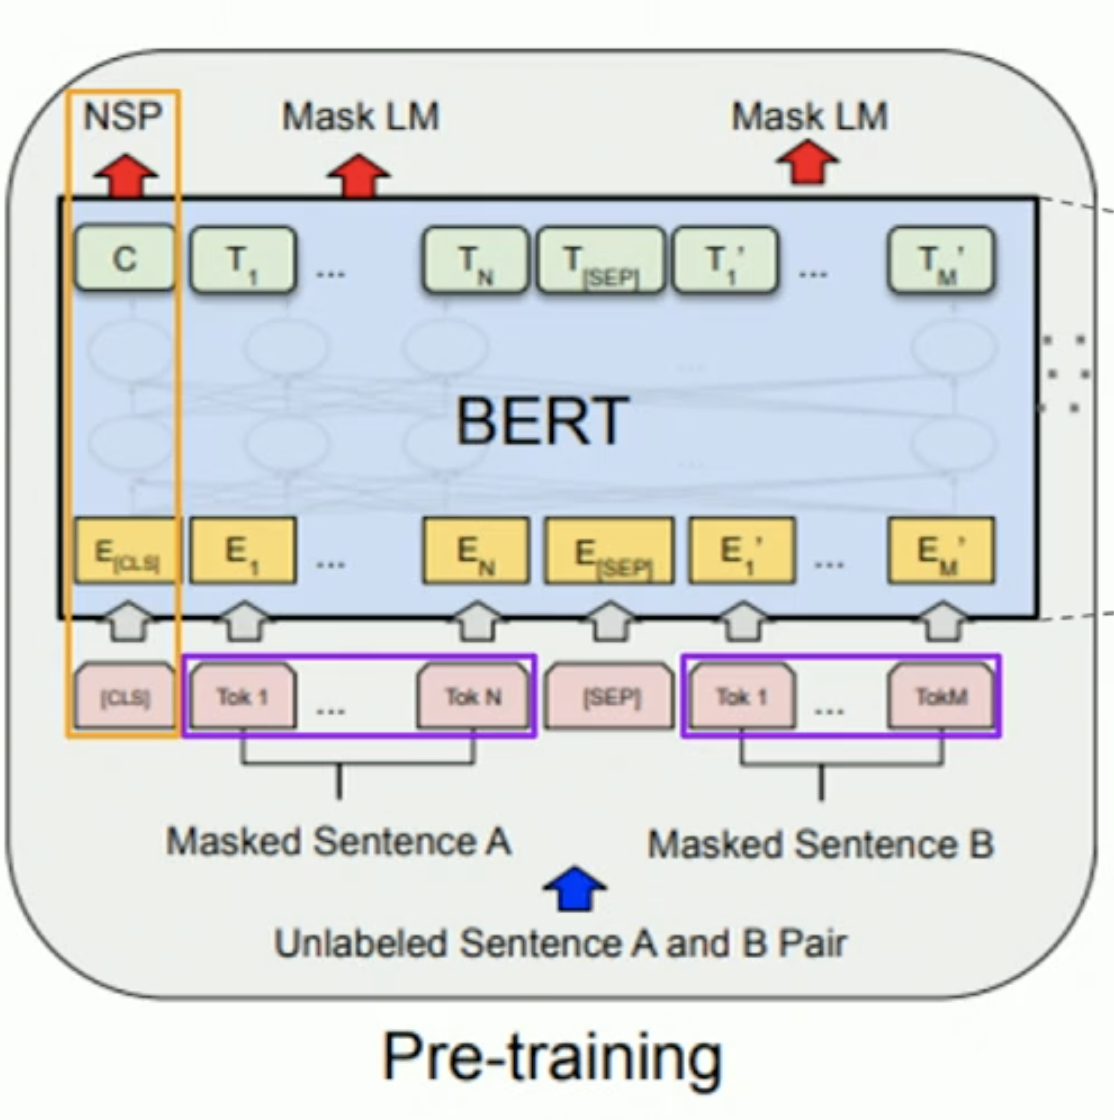
\includegraphics[scale=0.3]{images/BERT.png}
\end{center}

Then, pairs of sentences are passed in and the model must predict which sentence follows the other(done with the [CLS] token which is mapped to NSP), called the entailment prediction.  The goal of this is for BERT to learn sentence level representations of the data.  
\subsubsection{The GLUE Benchmark}
It is comprised of several different language tasks.
\begin{center}
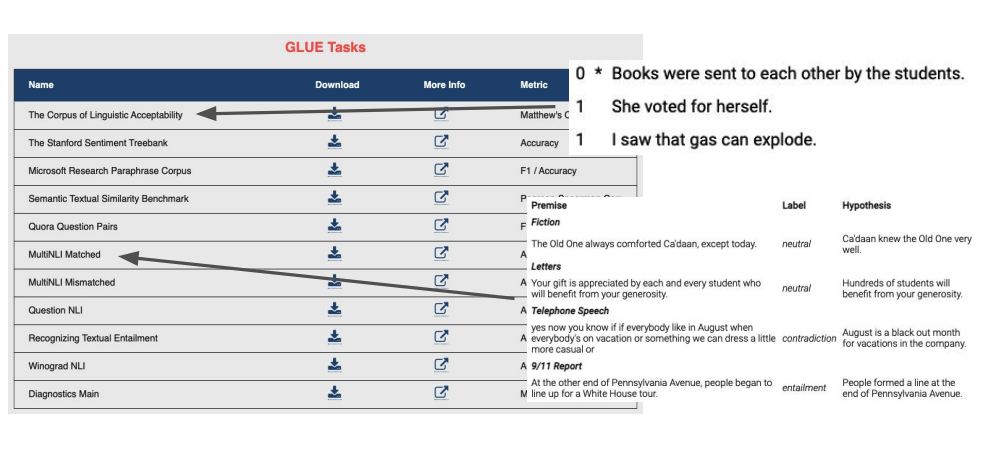
\includegraphics[scale=0.4]{images/GLUE.png}
\end{center}
  BERT does very well in these tasks upon Fine-Tuning.  After we use the pre-trained BERT model, we can fine tune in whatever way is dictated by the task to solve that particular task.  Since BERT architecture relies on tokenized inputs, all the different tasks can be solved using the fine-tuned BERT model. 
  \begin{center}
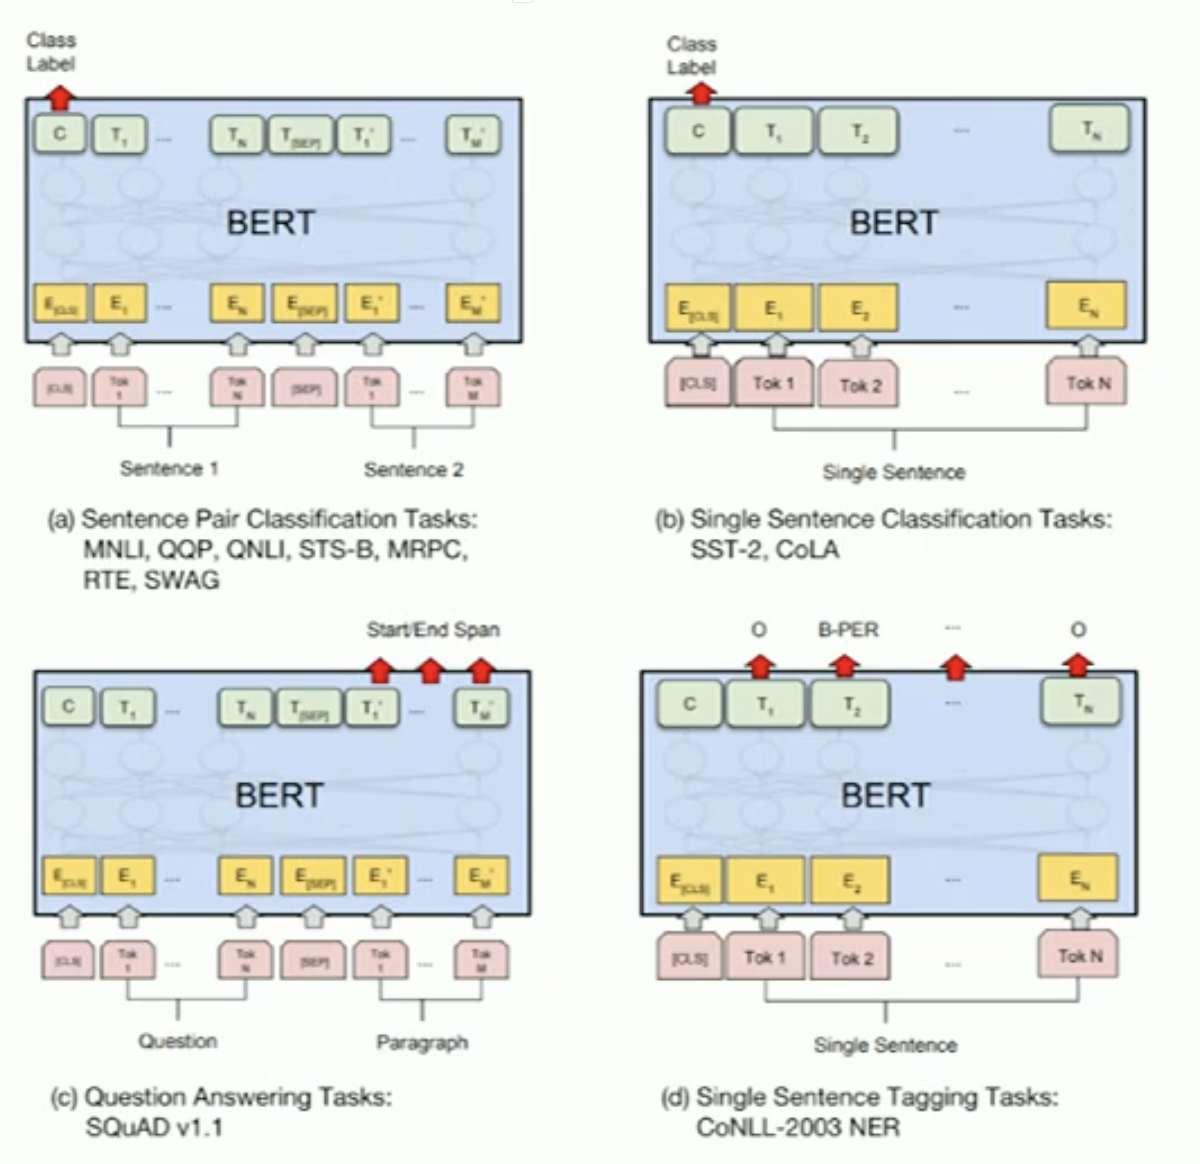
\includegraphics[scale=0.5]{images/gluetest.png}
\end{center}
\subsection{Encoder: Vision Transformer}
The input image is divided up into $16 \times 16$ patches and are treated as a sequence and pass it into a transformer to see what it could do.  
\begin{center}
\includegraphics[scale=0.3]{images/VIT.png}
\end{center}
\begin{itemize}
\item During training, the image is split into patches and projected down with a learned network(the first feed forward layer).
\item A ConvNet instead of a Linear Projection for the first layer also works well.
\item These are combined with the positional encodings and fed to the encoder(these are usually learned for Vision Transformers)
\item Then, a net on the first special position token is passed through a fully connected network which outputs logits, and we use cross-entropy loss and backpropagate the whole thing so that we can perform image classification.  
\end{itemize}
\begin{remark} Why do we need positional encodings?  Even though we want to mainly focus on local information, as we stack them deeper and deeper we are able to see non-local information, since the receptive field grows to the point where we can see things that are far apart.  We wouldn't be able to understand the ordering of the patches if we didn't have positional embeddings.  
\end{remark}
\subsection{Swin Transformer}
Swin stands for Shifted Window.  The original vision transformer considered $16 \times 16$ patches of the image and did self-attention on each of the $16 \times 16$ patches of the image.  But $16 \times 16$ is a fairly low resolution and we sometimes want more fine grained patches for certain tasks.  Note that the sequence-length is quadratic in the size of the patch, so if we divide $16 \times 16$ into $8 \times 8$, we halfed the height and width but quadrupled the number of patches.  
\begin{center}
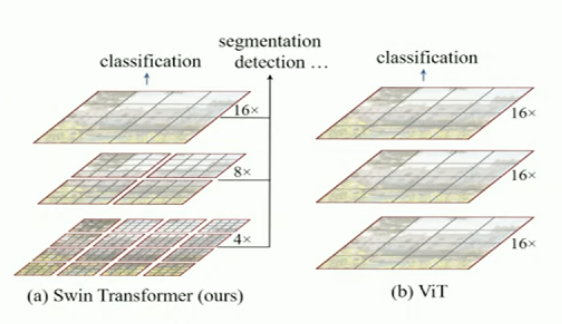
\includegraphics[scale=0.6]{images/swin.png}
\end{center}
Swin does smaller patches, but to fix the quadratic issue, they perform self-attention over a local region of the image that we have.  But this might not be able to address global dependencies.  This is handled through the shifted window:

\begin{center}
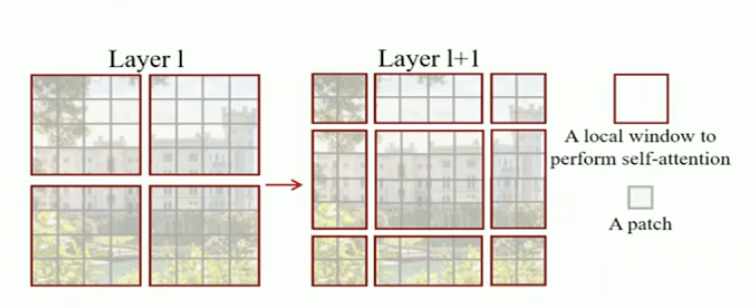
\includegraphics[scale=0.5]{images/shiftedwindow.png}
\end{center}
In the next layer, we shift over the window so that we can aggregate information over the whole image by stacking layers on top of each other.

\subsection{Unsupervised ViT}
The main idea behind this is \textbf{distillation}, where you have two ViTs and they both have no supervision, but if you get clever and train one to match the other(with certain inductive biases), you can get good an unsupervised training of a model that can be used later.  

\subsubsection{Masked Autoencoders}
This is the similar to what BERT is doing. We have an input image and we mask some amount of the image(usually around 75$\%$ of the image).  Using the unmasked patches, we pass them through a transformer encoder, map it back to the patches that weren't masked and mask tokens, and pass this to a decoder(not actually a transformer decoder).  
\begin{center}
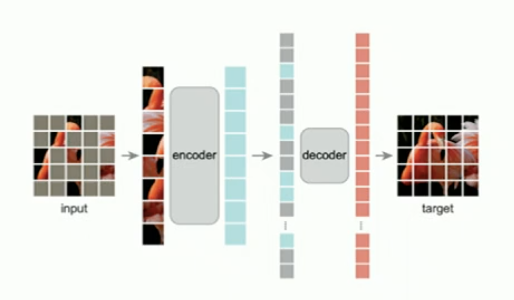
\includegraphics[scale=0.8]{images/masked-autoencoder.png}
\end{center}
\pagebreak
\section{03/14/2022 - Sequence-to-Sequence Models}
We are converting input sequences into output sequences.  The canonical example is \textbf{machine translation}, where we translate sentence $A$ into sentence $B$.  This is the main example that we focus on today. 

\subsection{Seq2seq Models}
We already discused several models for handling sequential data(RNNs, LSTMs, Transformers).  We also discussed cases where the input is not a sequence but the output is.  Now, we fill in the blanks for sequence input and sequence output tasks.

\begin{itemize}
\item Generally, we read in the entire input sequence before trying to generate the output sequence.  This is not always necessary, for example, we could have transformer-type architectures that translate sequences into new sequences with masking. 
\item We focus on many-to-many where we read in the entire input first.  
\end{itemize}

This is the canonical way of solving this problem and all seq2seq models follow the encoder-decoder architecture.
\begin{itemize}
\item The encoder reads in the input sequence and encodes it into a representation.
\item The decoder conditions on this representation in order to decode the output. 
\item Historically, both of these were LSTMs with separate parameters. 
\item Nowadays, they are both usually transformers.
\end{itemize}
\subsubsection{RNN(LSTM) seq2seq, basic}
We have a sentence "un chiot mignon".  We feed a token for each word and move to each word in the sentence.  Then, we pass it into a new decoder RNN by first giving it a <start> token and conditioned on the representation, we output probabilities of what the first word might be.  Then, we pass this back into the decoder to keep generating words in an auto-regressive fashion. We keep going until we see an <end> token.
\begin{center}
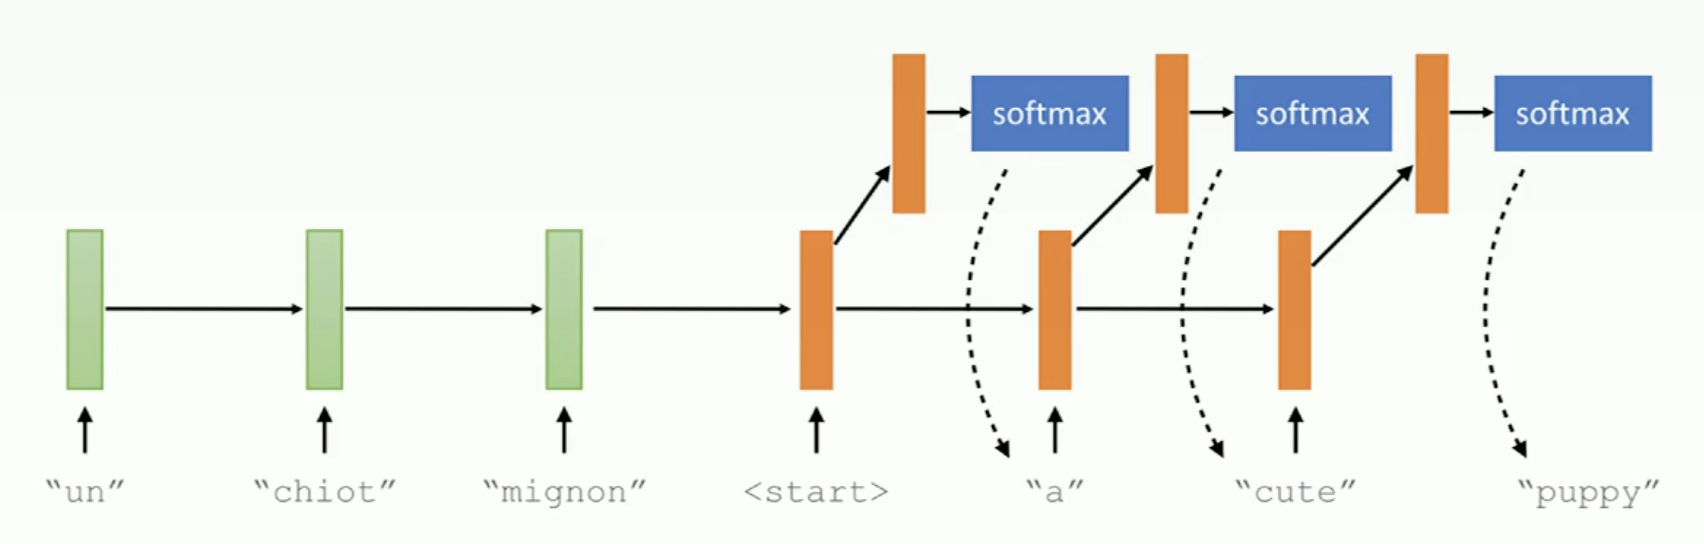
\includegraphics[scale=0.4]{images/basicseq.png}
\end{center}
\subsubsection{Multilayer RNNs}
A simple modification is to add more layers.  All of our layers pass into hidden states which correspond to better and better representations.  
\begin{center}
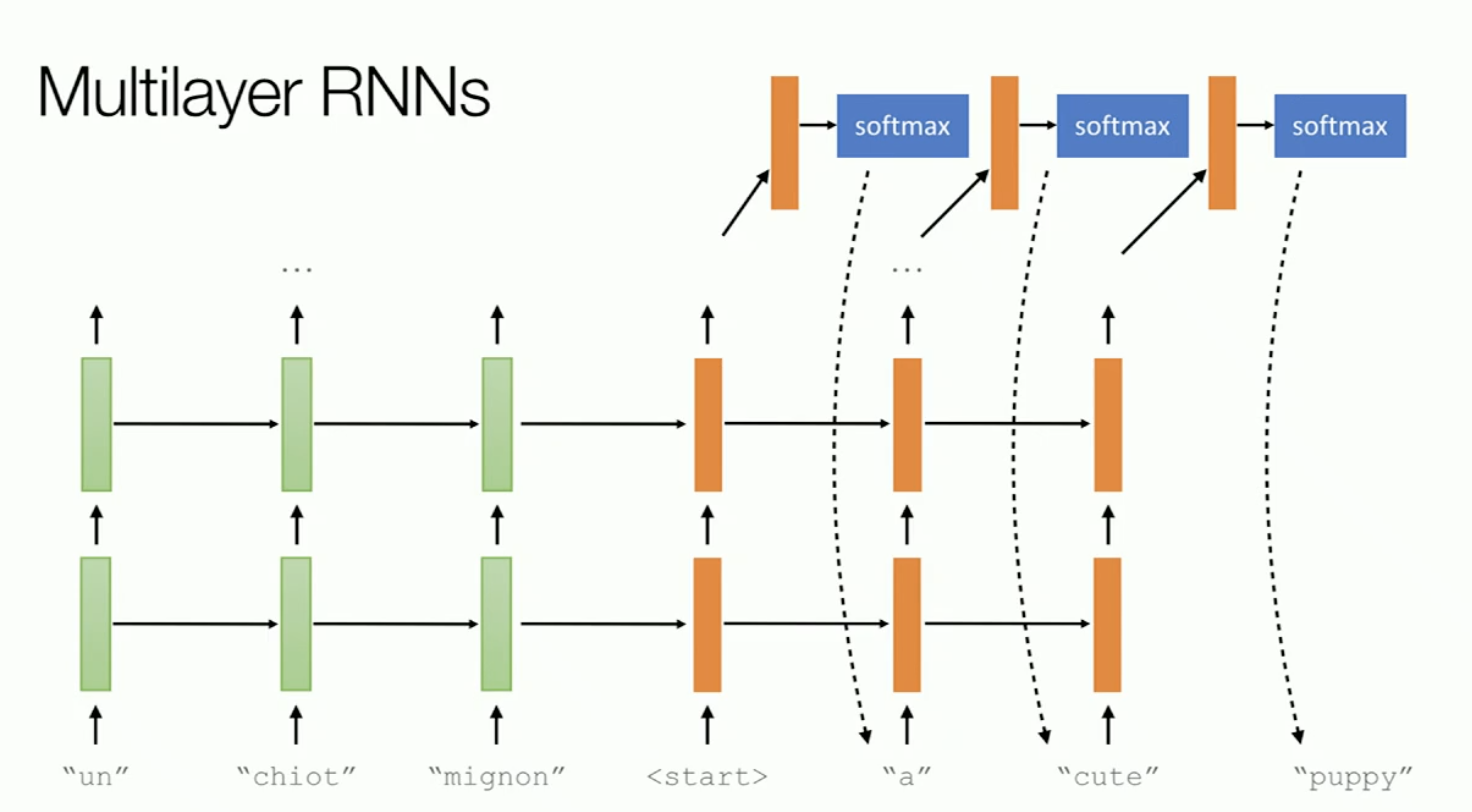
\includegraphics[scale=0.4]{images/multiseq.png}
\end{center}

What are some issues with the above models?
\begin{itemize}
\item We have the \textit{bottleneck problem}.  All information about the source sequence has to pass through a direct connection between the encoder and decoder, so the connection between the encoder and decoder is very crucial.  
\item This makes it difficult - for example, if the last word we want to decode corresponds to the first word.  The issue is that we saw a token whose information flow has to survive through all the different hidden states.
\end{itemize}
\subsubsection{Attention}
Now, we use attention to connect the encoder and decoder is a more direct way without relying on a single connection.  We make keys from each hidden state, and we treat the hidden states as values directly.   Then, we generate queries from the hidden states of the decoder and comparing these with the keys and values with a dot product giving us a similarity score.  Then, taking a softmax and taking a weighted sum, with all the values with the weights computed using the dot products, we obtain the representation that we use to generate the output at the particular timestep. 
\begin{center}
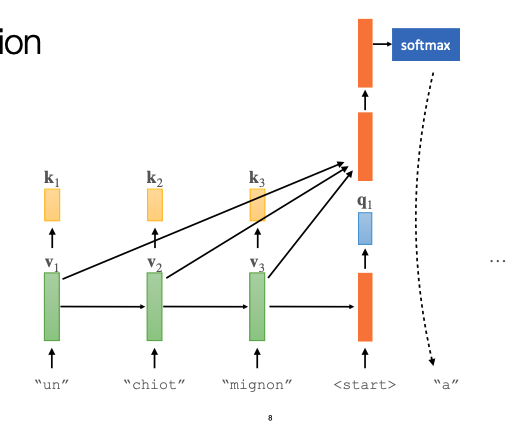
\includegraphics[scale=0.3]{images/rnn_attention.png}
\end{center}
\begin{itemize}
\item With attention, the direct connection between encoder and decoder becomes less important.
\item We can make the encoder a bidirectional RNN and attend over the outputs.  Attention allows the decoder to look at all the hidden states representations that the encoder is producing.  So we might get a better understanding of what a token means at a timestep by looking at the past and the future(one LSTM running forwards and backwards and concatenating representations).  The decoder still needs to be unidirectional since we generate in an auto-regressive manner.
\item The value function is the identity function in this case.  This is slightly different from before, where we learned the value function.  We also could have used a learned value function.
\item We could also make the key and query identity functions.  In that case, we are comparing the hidden states directly and based on those similarities, we generate the element to be used for the next timestep.  
\end{itemize}
\subsection{Seq2Seq Transformers}
Given an input sequence $X$, we learn a representation $Z$ from the transformer encoder.  Then, we have a separate decoder learning the output sequence which generates a sequence in an auto-regressive manner.
\subsubsection{Cross Attention Layers}
In the cross attention layer, we use the key and value from the transformer encoder and the queries from the decoder,masked self-attention.
\begin{center}
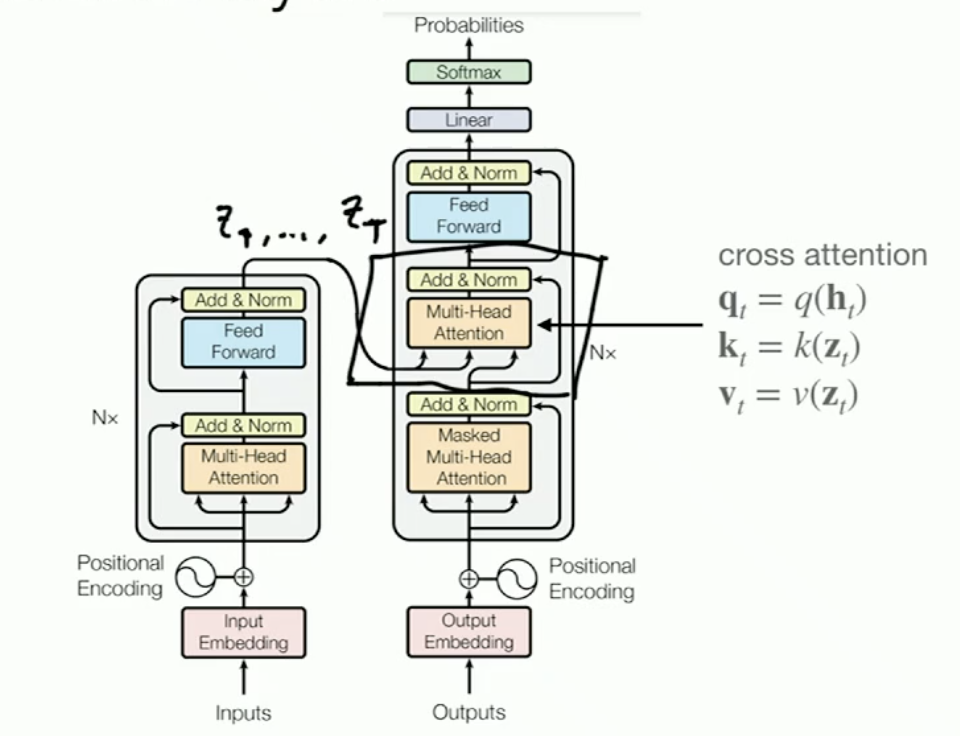
\includegraphics[scale=0.5]{images/cross.png}
\end{center}
\subsection{Recent seq2seq: T5}
\begin{itemize}
\item The text-to-text transfer transformer(T5) solves many different NLP tasks in a unified text input, text output framework.
\item We pass in an input sequence prepended with the actual task and these are uniformly handled and solved using T5.  
\item This is trained on C4 and achieves a number of competitive and state-of-the-art results.  
\end{itemize}
\begin{center}
\includegraphics[scale=0.6]{images/T5.png}
\end{center}
\pagebreak
\section{03/16/2022 - John DeNero: Neural Machine Translation}
\begin{itemize}
\item Text as input and text as output
\item Input and output have roughly the same information content
\item The output space is very large, but the output is more predictable than a language modeling task.
\end{itemize}
One issue is that there is variety in Human-Generated Translations.  This could be because of grammatical errors, different orderings of words, etc.  So we have issues even with the labels of our dataset.   
\subsection{Conditional Sequence Generation}
We estimate $P(e|f)$ from a sequence model $P(f, e)$.  To do this, we run an RNN over the whole sentence, which first computes $P(f)$, then computes $P(e, f)$.
\begin{center}
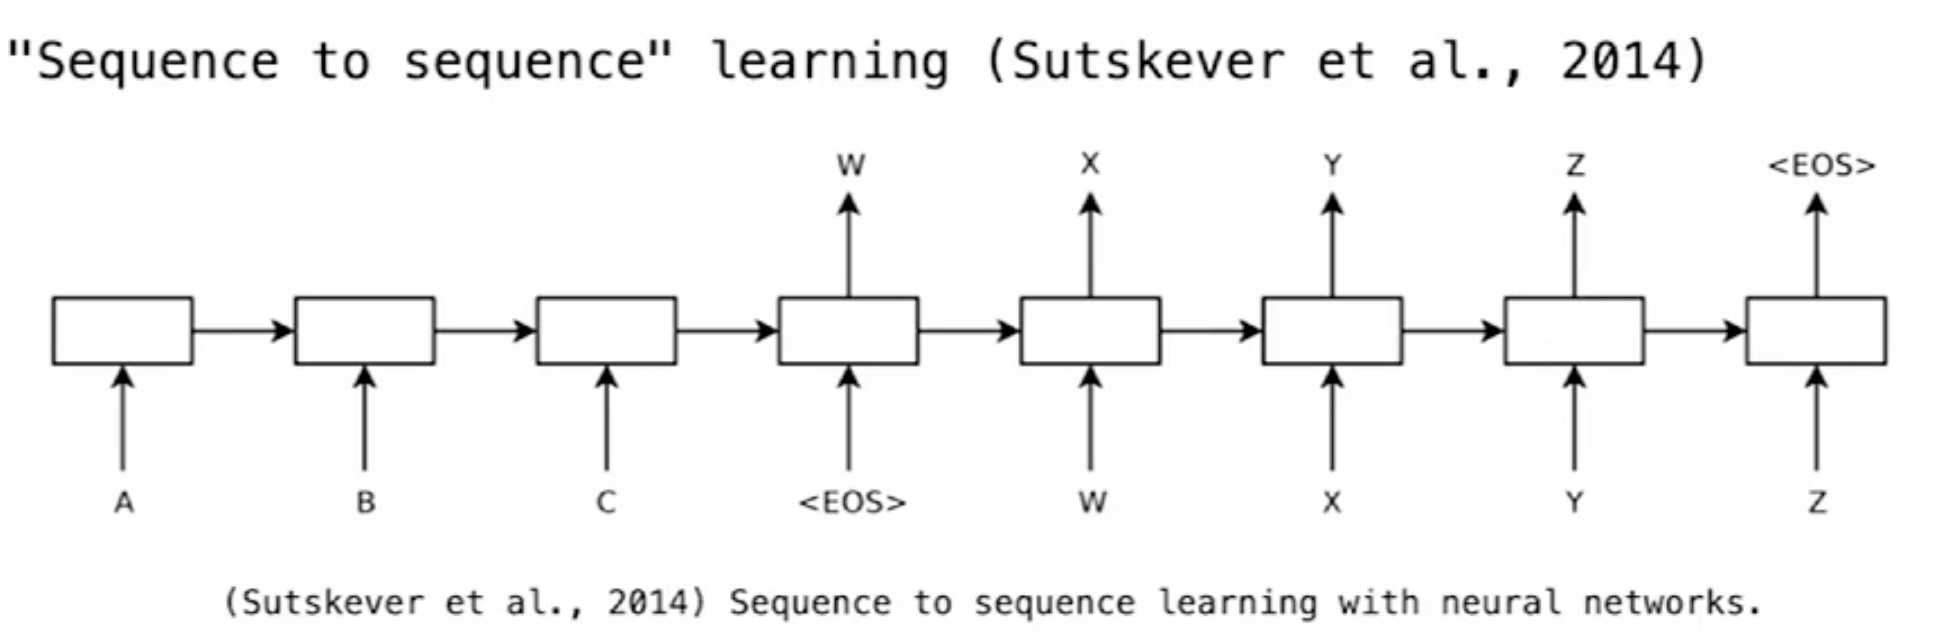
\includegraphics[scale=0.4]{images/sutskever.png}
\end{center}
We can do better by using an encoder-decoder model: different parameters or architectures for encoding $f$ and predicting $e$.

\subsection{Search Strategies}
\begin{itemize}
\item For each target position, each word is scored(alternatively, you could use a restricted list, but the quality degrades), and you choose the highest score.
\item Greedy decoding: extend a single hypothesis with the next word that has the highest probability. This will tend to have repetitions because it is not uncommon for a word to appear more than once causing a loop.
\item We want sequences with the highest probability, not just words.  To do this, we use Beam Search: Fixed number of partial translations(usually two), then prune.
\end{itemize}
\begin{center}
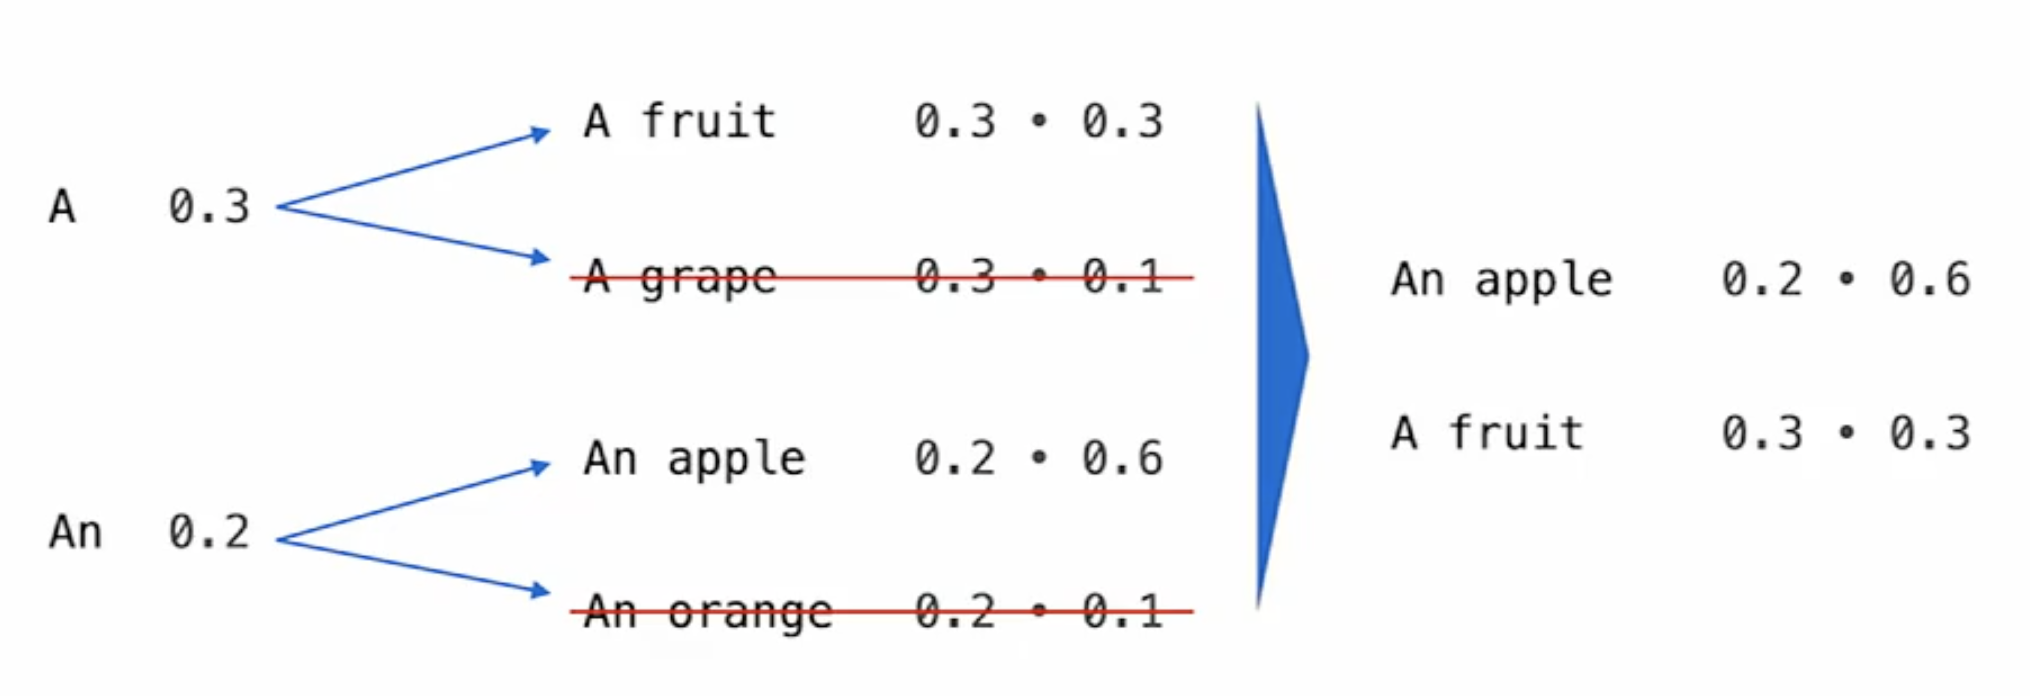
\includegraphics[scale=0.4]{images/beam.png}
\end{center}
In actually implementing Beam Search for Batch Decoding, we have the following:
\begin{center}
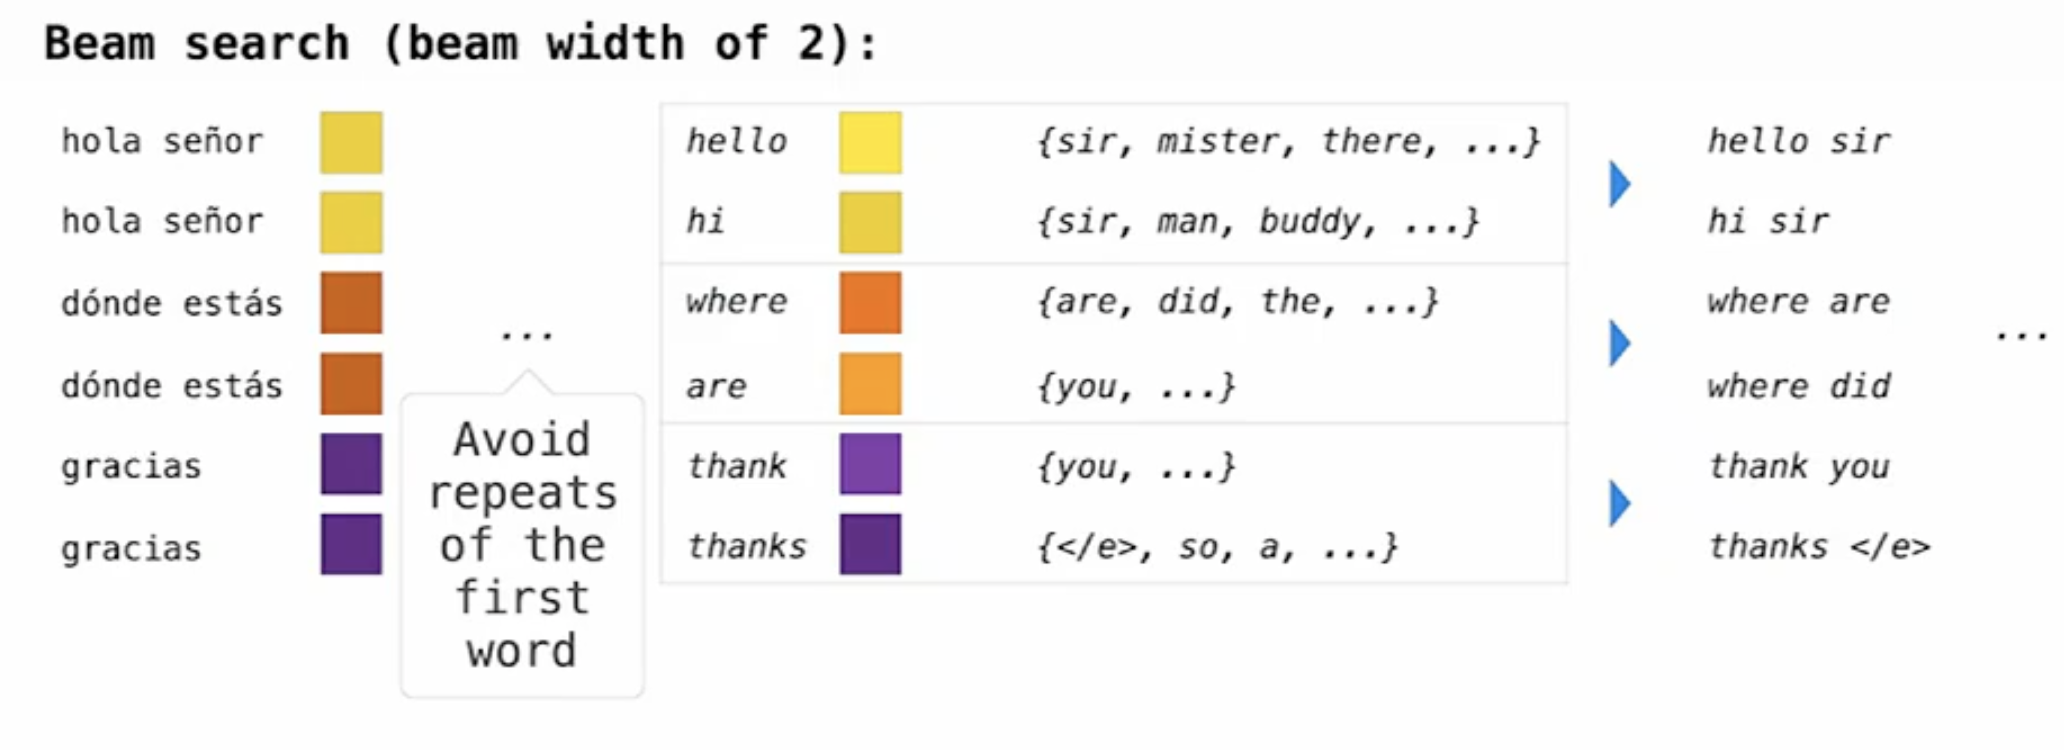
\includegraphics[scale=0.4]{images/beam2.png}
\end{center}
\begin{itemize}
\item We do something to make sure we don't pick the same word for both branches. 
\item  Then, we consider the scores for the top vocabulary options and choose the top two.  
\end{itemize}
Generally, NMT models prefer translations that are two short.  
$$s(e) = \sum_{i=1}^m \log P(e_i | e_{1 : i}, f).$$
\begin{itemize}
\item The model is made up of a product of things less than $1$, so the longer the sequence, the smaller it tends to be.  
\item Another explanation has to do with how they are trained, we don't just maximize the probability of unseen data, but we hold out the probability mass with unseen things like dropout, etc.  It forces the probability terms to be smaller than they should be, and multiplying things that are shorter than they should be results in smaller sentences. 
\item "For more than 50\% of sentences, the model in fact assigns its global best score to the empty translation" (Stahlberg and Byrne, 2019)
\end{itemize}
To deal with these issues, we use alternative scorings on the beam:
\begin{center}
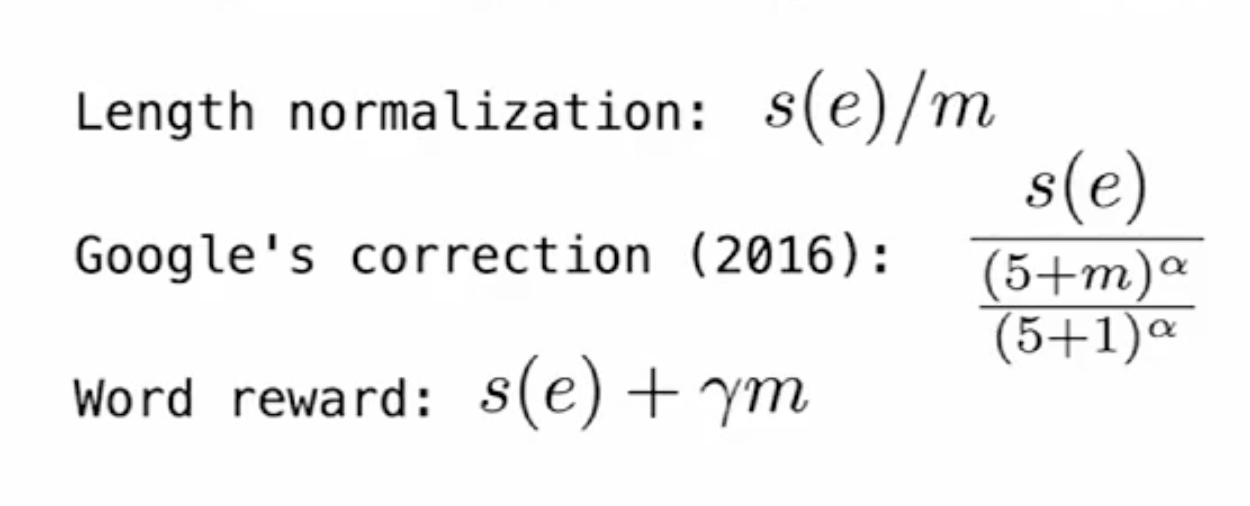
\includegraphics[scale=0.4]{images/beamscore.png}
\end{center}

\subsection{Training Loss}
We do something called \textbf{teacher forcing}: during training, only use the predictions of the model for the loss, not for the input.  

One hack is label smoothing: update toward in a distribution in which 0.9 is assigned to an observed word and 0.1 probability is decided uniformly among the other words.  

\subsection{Subwords}
The sequence of symbols that are embedded should be common enough that an embedding can be estimated robustly for each, and all symbols have been observed during training:
\begin{itemize}
\item Solution 1: Symbols are words with rare words replaced by UNK.  
\begin{itemize}
\item Replacing UNK in the output is a new problem(like alignment).
\item UNK in the input loses all information that might have been relevant from the rare input word(tense, length, POS)
\end{itemize}
\item Solution 2: Symbols are subwords
\begin{itemize}
\item Byte-Pair encoding: splits a word into subwords
\item Other techniques that find common subwords aren't reliably much better.
\item Training on many sampled subword decompositions can improve out-of-domain translations. 
\item If there is only one way of splitting up a word, we might miss other ways of splitting a word that is better for translation.
\end{itemize}
\end{itemize}
\subsubsection{Byte-Pair Encoding}
\begin{center}
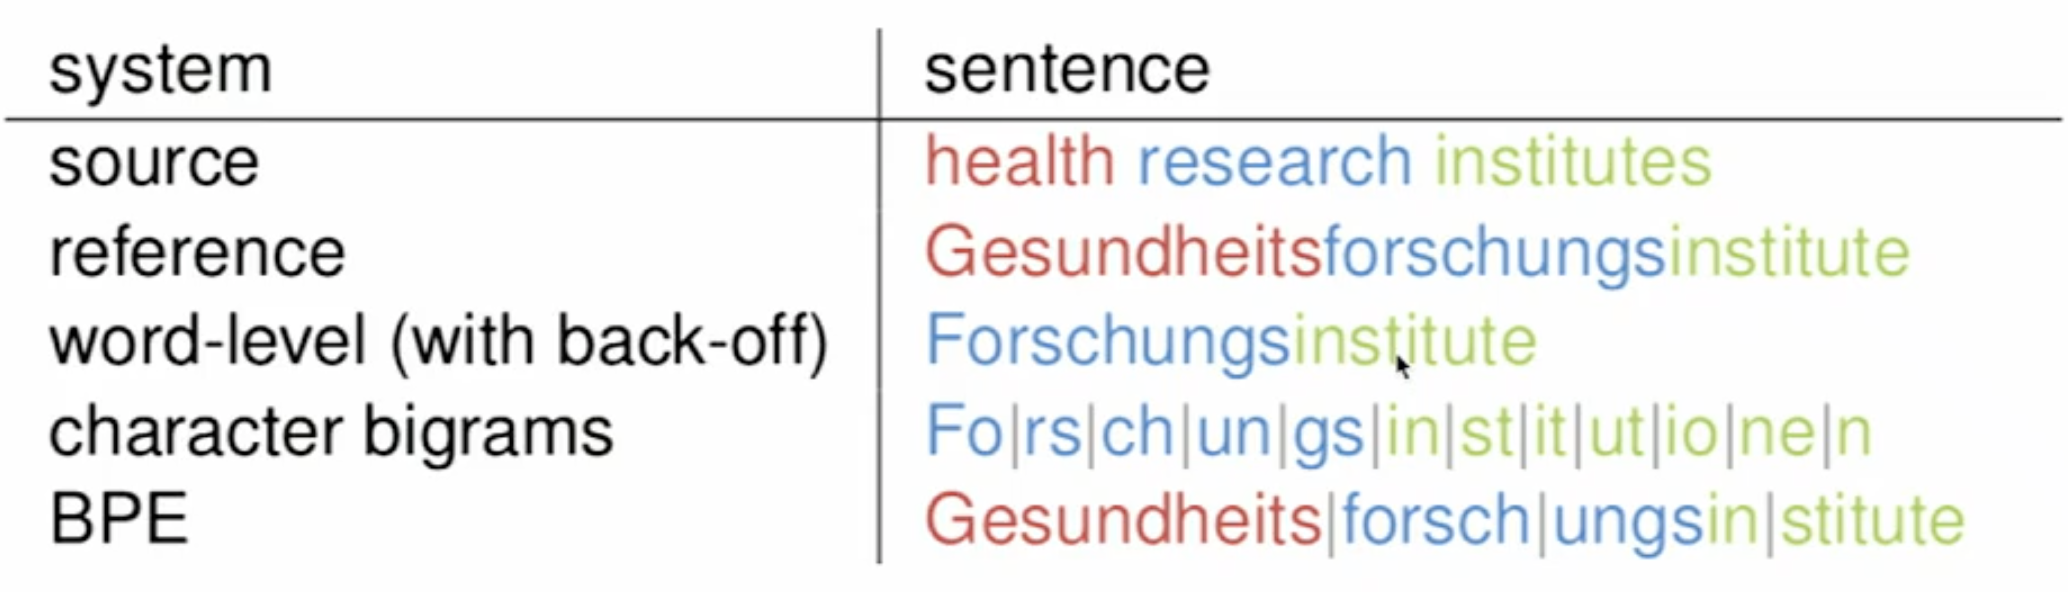
\includegraphics[scale=0.4]{images/bpe.png}
\end{center}
You start by splitting each word into characters.  Then you find the most frequent pairs of characters and turn that into a new character.  Repeat.
\subsection{Back Translations}
One trick is to synthesize an en-de parallel corpus by using a de-en system to translation monolingual de sentences.  This can help if the de sentences are already in a en-de parallel corpus!
\pagebreak
\section{03/28/2022 - Distribution Shift}
Today, we will be talking about \textbf{distribution shift}: when the test data comes from a different distribution than the training data.  The real world is full of distribution shift - the world changes all the time and it is common that the training data becomes outdated or is not representative of the full picture.  Usually, it is benign, but it can be harmful sometimes.  

This can cause accuracy to go down, but it can cause other degradations:
\begin{itemize}
\item worse calibration
\item worse fairness: worse for particular users
\end{itemize}
Most of these examples come from computer vision(image classification in particular).
\subsection{Risk}
\newcommand{\E}{\mathbb{E}}
Recall, we defined \textbf{risk} $R(\theta) = \E[\ell(\theta; X, Y)]$.  We also defined empiral risk $\hat{R}(\theta) = \frac{1}{N} \sum_{i=1}^N \ell(\theta; x_i, y_i)$, a monte carlo estimate of the true risk.  
\begin{itemize}
\item Supervised learning is refered to as empirical risk minimization(ERM).
\item Why and when does it make sense to use this as an objective?
\end{itemize}
\subsubsection{The ERM Assumption}
ERM is based on the assumption that the test data distribution is the same as the training data distribution.  Under this assumption(and good validation, regularization), we can derive \textit{generalization bounds} of how well we expect models to generalize to new data, and even for deep neural networks! 

This assumption is used by almost all supervised learning methods, and it is referred to as "the big lie of machine learning" by Prof. Zoubin Ghahramani.  This is because it is very rarely the case that training and test data match perfectly. There are many cases where it "almost" holds, but there are scenerios that do not generalize at all.
\subsection{Distribution Shift in the Real World}
Distribution shift in the real world is the norm, not the exception.  But we need to consider whether or not it will be a problem in our application.
\begin{itemize}
\item If it is in a continuous deployment setting, the model will likely encounter future scenarios not represented in training data.  
\begin{center}
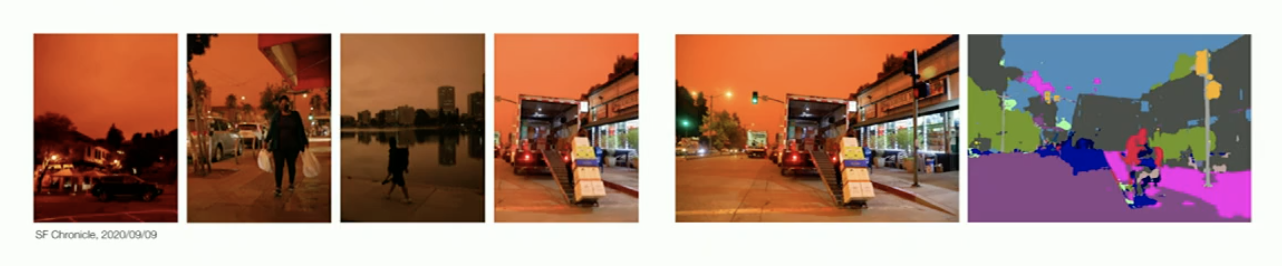
\includegraphics[scale=0.6]{images/dshift.png}
\end{center}
\item If the model interacts with end users, some users will be atypical and challenge the model in strange ways. 
\end{itemize}
\subsection{Distribution Shift Benchmarks}
We have multiple objectives:
\begin{itemize}
\item Benchmarks that are diverse and representitive or real applications.  If we had synthetic benchmarks then we run into the issue where we design methods that overfit to the synthetic benchmarks but don't perform well in the real world. 
\item Benchmarks that are easy to use and evaluate on.
\end{itemize}
\subsubsection{ImageNet Challenge Test Sets}
This is a popular way to test model \textbf{robustness} to different distribution shifts.  The test sets are designed to stress test models by simulating extreme or highly unusual events(that are still plausible).
\begin{center}
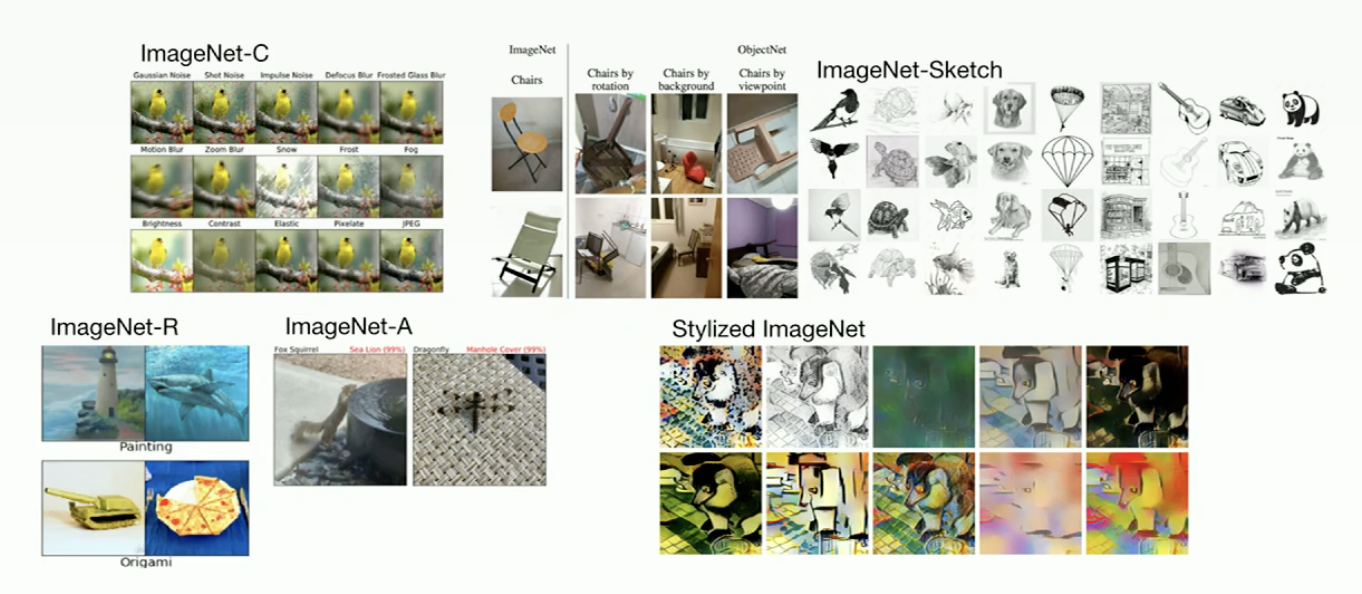
\includegraphics[scale=0.6]{images/ima.png}
\end{center}
They contain the same classes as ImageNet so any model trained on ImageNet can be evaluated on these test sets.  
\subsubsection{WILDS Benchmark}
\begin{itemize}
\item Having easy to use and standardized challenge test sets are important but they might not be the full picture. 
\item We are limiting ourselves to just image net, which does not cover the entire space.  
\end{itemize}
WILDS aims to curate a suite of problems that faithfully represent how distribution shift manifests itself in real world applications.
\begin{center}
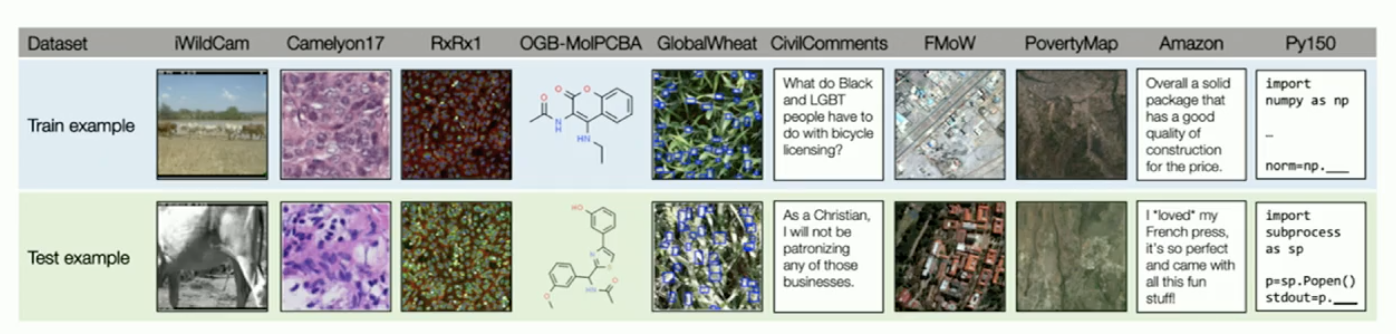
\includegraphics[scale=0.6]{images/wilds.png}
\end{center}
\subsection{NLP: ANLI Dataset}
\begin{itemize}
\item Natural language inference is the task of determining if a premise sentence and hypothesis sentence are related through contradiction, neutrality, or entailment.  This is part of the GLUE benchmark.
\item The \textbf{adversarial natural language inference (ANLI)} dataset consists of crowd-sourced hypothesis written to fool state-of-the-art pre-trained models.
\item To construct the dataset, an annotator is asked to write a hypotehsis given a premise and a condition.
\begin{itemize}
\item If the model corrects predicts the condition, the annotator tries again.
\item If incorrect, hypothesis is verified by other annotators. 
\end{itemize}
\end{itemize}
\subsection{Robustification}
How do we make models more robust?  For WILDS, the training dataset comes with more info that we can leverage.  But for image set, we don't get additional information for training.  Some general techniques that have proven useful are:
\begin{itemize}
\item Train larger models on larger, more diverse datasets
\item Using heavy data augmentation and alternate/additional training objectives. 
\end{itemize}
\subsubsection{Train on Larger Datasets}
Does this improve "robustness"?  Now, the test dataset is less out of distribution(OOD), so is the model more robust or have we just captured a training sample that better covers the test data. 
\begin{center}
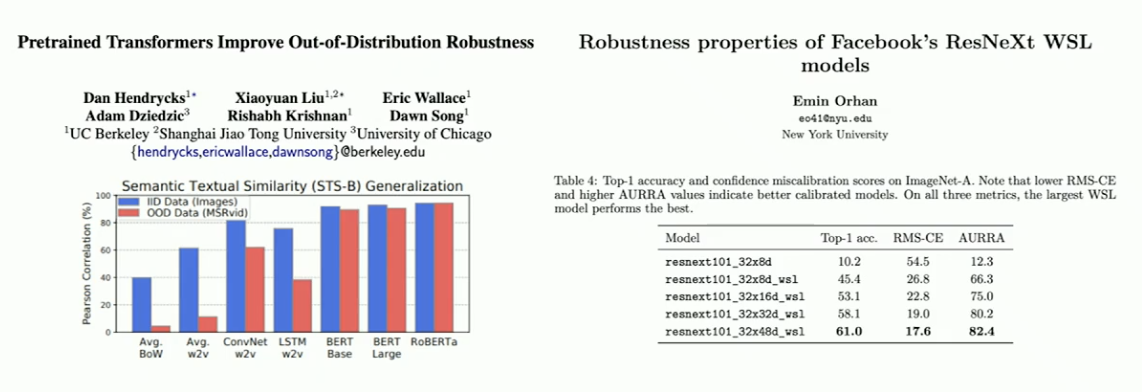
\includegraphics[scale=0.8]{images/large.png}
\end{center}

\subsubsection{Data Augmentations}
Some techniques are:
\begin{itemize}
\item Mixup: produce element-wise convex combinations of datapoints and improve corruption robustness.
\item AutoAugment: learns complex augmentation strategies from basic ones by training tens of thousands of deep neural networks.  This is a very expensive strategy but not a bad strategy. 
\item AugMix: mixes together random augmentations using ones from AutoAugment
\item PixMix: Mixes in images from a dataset(such as fractals) and mixes it together resulting in consistently good performance across several metrics. 
\end{itemize}
\subsubsection{Masked Autoencoders}
The current state of the art numbers are trained with ViT models with a pretrained masked autoencoding objective. 
\begin{center}
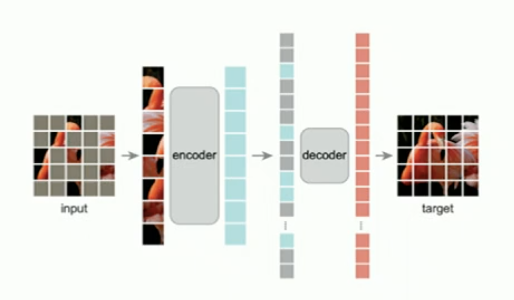
\includegraphics[scale=0.9]{images/masked-autoencoder.png}
\end{center}
Then, we find tune the encoder on ImageNet.  Supervised learning on the original ImageNet training set after this pretraining leads to the best results amongst models that do not get additional data.
\begin{center}
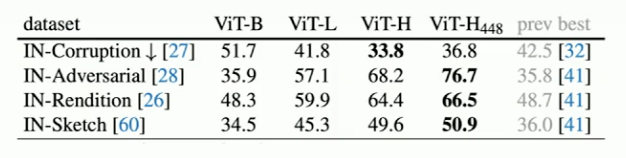
\includegraphics[scale=1]{images/masknumber.png}
\end{center}
\subsection{Anomaly Detection}
\begin{itemize}
\item If the system can detect an anomaly, then it might be able to enter some conservative mode or a fail-safe to avoid catastrophic errors. 
\item Detect malicious use of ML systems(hackers)
\item Detect potential dangers, like dangerous novel microorganisms.
\end{itemize}
\subsubsection{Implementation}
\begin{itemize}
\item Assign an anomaly score to every input $x$.  We only do this for inputs because we want to be able to do this at test time as well.  Higher scores are more anomalous.
\item What if we learned a model of $p(x)$( a generative model) and treat $x$ as anomalous if it has low $p(x)$?
\begin{itemize}
\item This does not currently work well since learning models of $p(x)$ is very difficult.  
\item It is also not sure if models using $p(x)$ or $\log p(x)$ is actually that well-framed of an idea to detect anomalies.  
\item Modern deep generative models still do poorly at anomaly detection using the scheme for complex input spaces.
\end{itemize}
%\item There are some ways to make deep generative models useful, but they are more complex and require additional assumptions.
\end{itemize}
\subsubsection{A Simple Baseline}
\begin{itemize}
\item Doesn't involve training a generative model
\item Use the model's confidence $\max_k p_\theta(y = k | x)$ to detect anomalies.
\item Specifically, we use the score $- \max_k p_\theta(y = k | x)$.  We may also use $-\max_k z_k$, the negative of the max logit for some situations.
\item The simple baselines work well across CV, NLP, speech recognition, classifications, but it cannot detect adversarial examples.
\item Some more examples include likelihood ratios, outlier exposure, virtual logit matching.
\end{itemize}
\subsubsection{Benchmarks for Anomaly Detection}
\begin{itemize}
\item There is a much larger search space for constructing anomaly detection benchmarks - we train a model on one dataset and treat any other data as anomalous.
\item Example: train on CIFAR-10, evaluate on SVHN
\item Example: train on CIFAR-10, evaluate on CIFAR-100
\item Example: train on ImageNet-22k, evaluate on Species
\end{itemize}
\subsubsection{Evaluting Binary Classifiers}
\begin{itemize}
\item We can think of anomaly detection as binary classification, since we have anomalous or not.
\item What might be the issue of just considering accuracy?  Class imbalance: What if we have 1 anomaly, 99 normal.  The model that always predicts normal has 99\% accuracy, but is not a good detector.
\item So we need more detailed metrics, true positive, false positives, true negatives, false negatives.  
\end{itemize}
\pagebreak
\section{04/04/2022 - Adversarial Examples}
\subsection{Test time Adaptation}
\begin{itemize}
\item We talked about heuristic techniques like scaling up datasets and using data augmentation techniques.  But this all happens at training time.
\item Are there training time techniques to adapt to shift at test time using available information?  Assume we have access to and can change the model's parameters, or we have other means of augmenting the predictions.
\item We can assume we have multiple test points, from which we can estimate statistics of the underlying test distribution, and adapt to that distribution.
\item if there is a label shift($p(x | y)$ is the same but $p(y)$ changes), we can change the threshold for predicting various classes according to how the label should change.  We can estimate this using the confusion matrix.  
\end{itemize}
\subsubsection{Methods for Test-time Adaptation}
\begin{itemize}
\item Batch Norm adaptation: leave the batch norm layers in training mode at test time.  This way we recompute statistics that we use for normalization at the test time.
\item Self-supervised learning: have a loss function that only depends on inputs and construct fake labels based on auxiliary tasks that we define.  For example: rotation prediction, entropy minimization.
\begin{center}
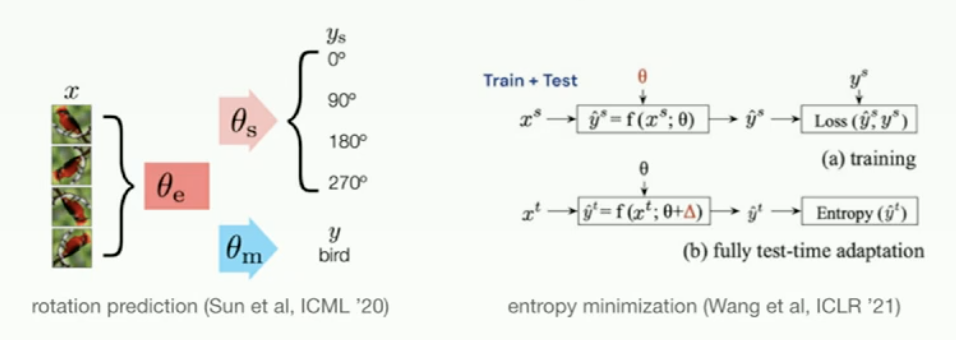
\includegraphics[scale=0.7]{images/selfsuper.png}
\end{center}
\end{itemize}
\let \mc \mathcal
If we have a standard model $g: \mc X \to \mc Y$, we can think of the adapted model as $f: \mc X \times \mc P_x \to \mc Y$, where $\mc P_x$ is a distribution that the input comes from.  In practice, we can estimate $\mc P_x$ with $(x_1, \dots, x_k)$.
\subsection{Adversarial Robustness}
We have an adversarial distortion that is carefully crafted to be imperceivable to the human eye but cause the model to predict a different layer.  These are models that have not been trained to handle adversarial examples.
\begin{center}
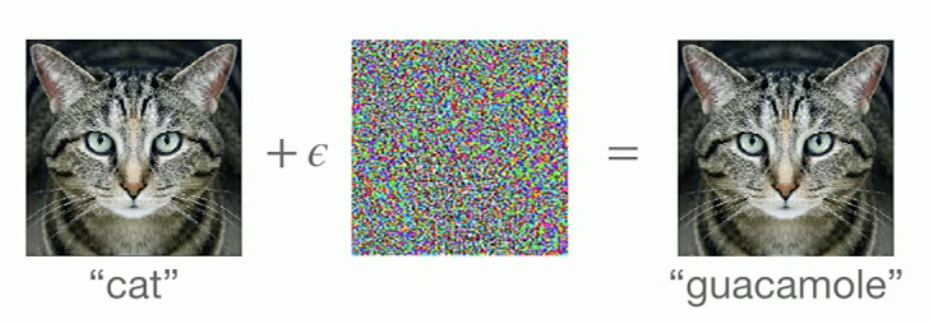
\includegraphics[scale=0.6]{images/adversary.png}
\end{center}
Now, we can mostly train against imperceptible distortions.
\subsubsection{Modern Adversarial Distortions}
In the modern examples, we have changes that are perceivable to the human eye, but the underlying class in unchanged.  This is not good either because we don't see a difference in the class but a large degradation in the image, but it will fool robustly trained classifiers.   
\begin{center}
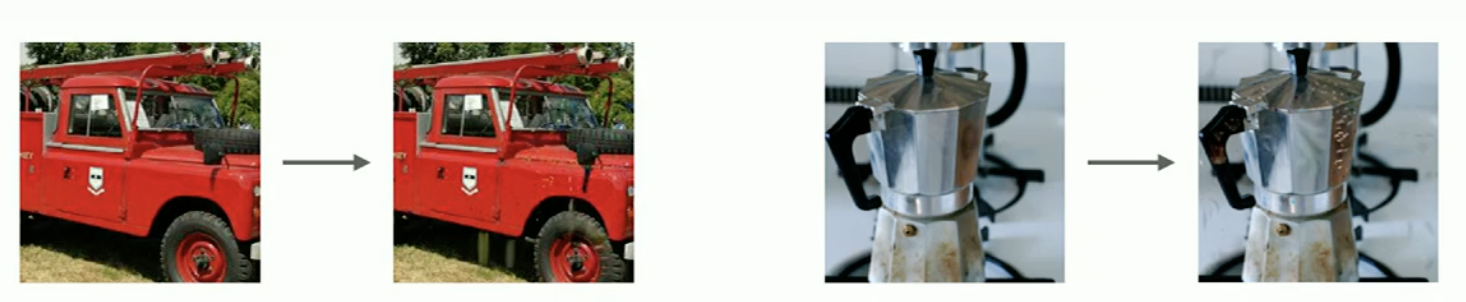
\includegraphics[scale=0.4]{images/moderndist.png}
\end{center}
Modern networks can be make robust to imperceptible distortions, but they are not robust to perceptible distortions.
\subsubsection{Fooling Binary Logistic Regression}
Suppose we have the model 
$$f_\theta(x) = \frac{\exp \theta^T x}{1 + \exp \theta^T x}.$$
If we say that we can change the inputs to $x + \epsilon$ with $\|\epsilon\|_\infty \le 0.5$, we can completely change the prediction of the model:

\begin{center}
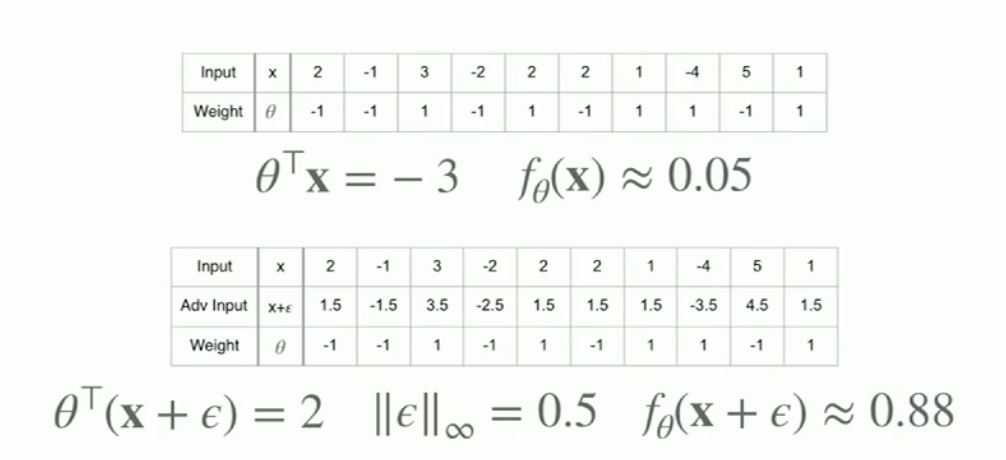
\includegraphics[scale=0.5]{images/binary.png}
\end{center}
\begin{itemize}
\item The comulative effect of many small changes made the adversary powerful enough to change the classification decision.
\item Adversarial examples exist for non deep learning models. 
\end{itemize}
\subsection{Adversary Threat Models}
It hopes to make assumptions about what the adversary looks like and what they are capable of.
\begin{itemize}
\item A simple model is to assume the adversary has an $\ell^p$ attack \textit{distortion budget} $\epsilon$: for some $p, \epsilon$, $\|x_{adv} - x\|_p \le \epsilon$.
\item Not all distortions have small $\ell^p$ norm, for example rotations.  But this is usually tractable to study.
\item The goal is to find a distortion $\delta$ to maximize the loss subject to the budget $$x_{adv} = x + \argmax_{\delta: \|\delta\|_p \le \epsilon} \ell(\theta; x + \delta, y).$$
\end{itemize}
\subsubsection{Fast Gradient Sign Method(FGSM)}
One simple attack: 
$$x_{FGSM} = x + \epsilon \sign(\nabla_x \ell(\theta; x, y)).$$
In this case, $\|x_{FGSM} - x\|_\infty = \epsilon$. If the gradient is accurate, the moving in the positive direction increases the loss and vice versa, so we go in the final direction that maximizes the overall loss.

The attack is called fast because it only uses a single gradient ascent step.  Nowadays, this is easy to defend against.  
\subsubsection{Projected Gradient Ascent(PGD)}
PGD uses multiple gradient ascent steps so is more powerful than FGSM.  How it works with $T$ steps and $\ell^\infty$ budget $\epsilon$
\begin{enumerate}
\item Randomly initialize a perturbed image $\tilde{x} = x + n$ where $n_i \sim \mc U[-\epsilon, \epsilon]$ and initialize $\delta = 0$.
\item for $t = 1, \dots, T$, set $\delta = \operatorname{clip}(\delta + \alpha \sign(\nabla_\delta \ell(\theta; \tilde{x} + \delta, y)), - \epsilon, \epsilon)$.
\item Set $x_{PGD} = \tilde{x} + \delta$.
\end{enumerate}
\subsection{Adversarial Training}
A common procedure is as follows:
\begin{enumerate}
\item Sample a minibatch $(x^{(1)}, y^{(1)}), \dots, (x^{(B)}, y^{(B)})$.
\item Create $x_{adv}^{(i)}$ from $x^{(i)}$ for all $i$.
\item Optimize the average training loss on these adversarial training examples.
\end{enumerate}
The downside of this is that AT can reduce accuracy on nonadversarial examples by 10\%. 
\subsubsection{Untargeted vs. Targeted Attacks}
So far, we have assumed untargeted attacks which try to maximize the loss.  By contrast, a targeted attack optimizes examples to be misclassified as a predetermined target $\tilde{y}$.  Targeted attack evalution is standard for ImageNet because there are many similar classes:
\begin{center}
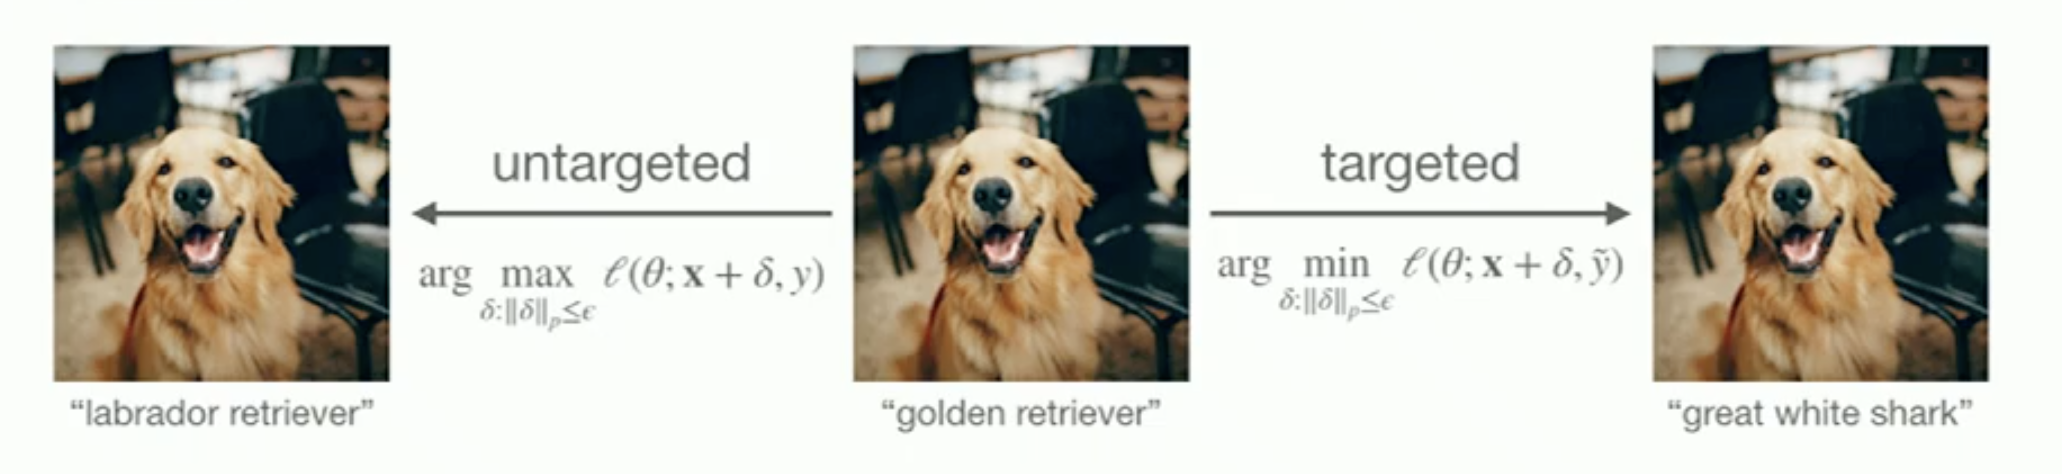
\includegraphics[scale=0.4]{images/target.png}
\end{center}
\subsubsection{Transferability of attacks}
\begin{center}
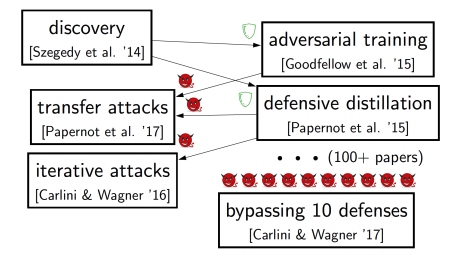
\includegraphics[scale=0.4]{images/armsrace.png}

\textit{The adversarial arms race}
\end{center}
An example crafted for one model can potentially be used to attack different models. For example, given $M_1, M_2$ neural network models, $x_{adv}$ designed for $M_1$ can sometimes result in a high loss for $M_2(x_{adv})$ even if $M_2$ is a different architecture.

The transfer rates can vary greatly, but even moderate amounts of transferability demonstrate that adversarial failure modes are somewhat shared across models.  Consequently, an attacker does not need access to a model's parameters or architectural information to try to attack it. 
\subsubsection{Using Larger and More Diverse Data}
\begin{itemize}
\item Adversarial robustness scales slowly with dataset size
\item Adversarial pretraining on a larger training set has been shown to help: to increase CIFAR-100 robustness, adversarially pretrain on ImageNet.
\end{itemize}
\subsubsection{Data Augmentation}
One particularly effective technique, combined with adversarial training with a parameter exponential moving average is \textbf{CutMix}.
\begin{center}
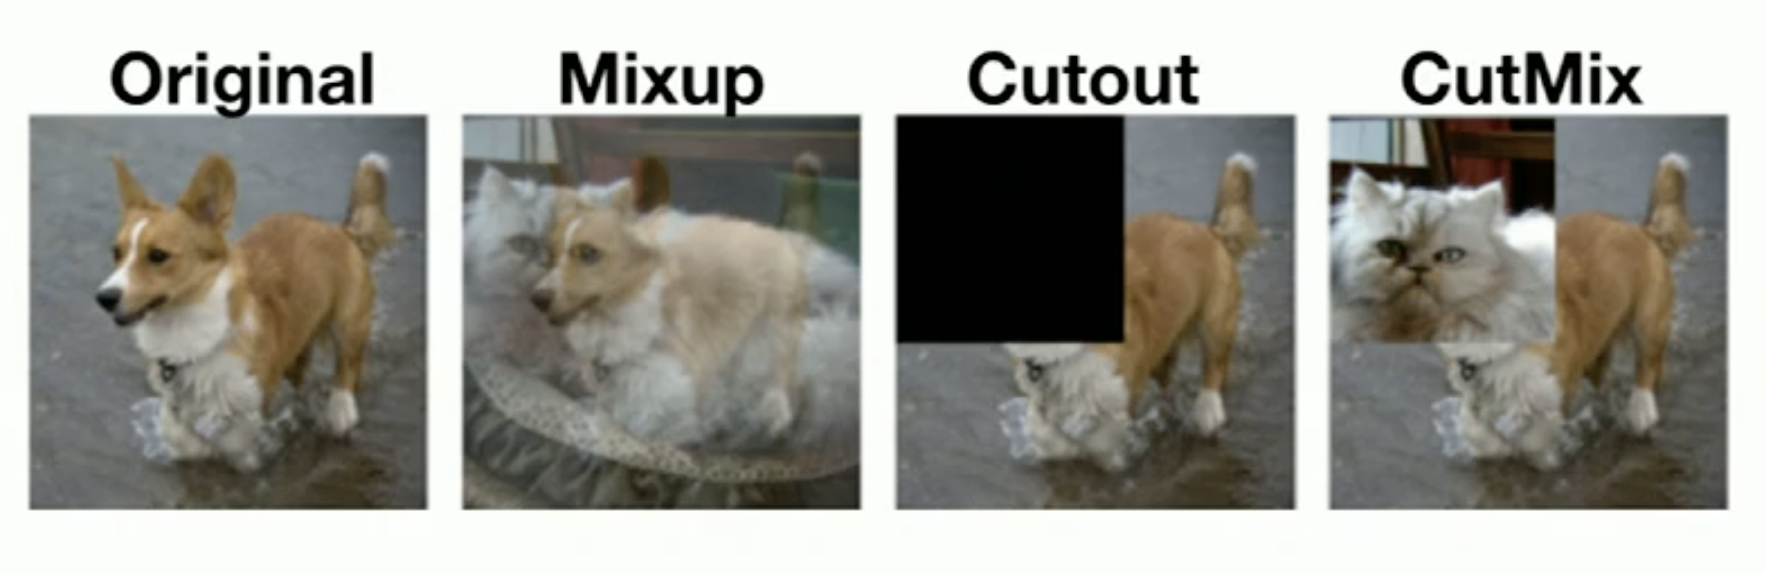
\includegraphics[scale=0.3]{images/cutmix.png}
\end{center}
\subsubsection{Choice of Activation Functions}
Sharp activations such as ReLUs make AT less effective since gradients are less conditioned, so by improving gradient quality for the attacker and network optimizer, smooth activiations like GELUs improve adversarial training. 
\subsection{Unforeseen Adversaries}
Models are far less robust to attacks they are not trained against. To estimate robustness to unforeseen attacks,we should measure robustness to multiple attacks not encountered during training
\begin{center}
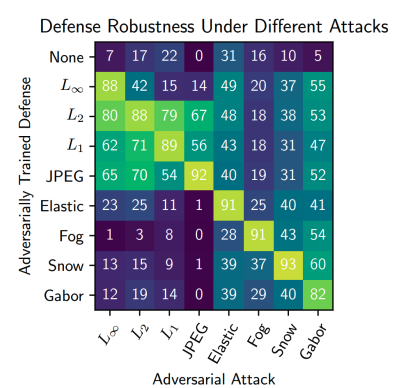
\includegraphics[scale=0.6]{images/robustmatrix.png}
\end{center}
 \pagebreak
\section{04/06/2022 - Generative Models}
Some examples we have seen before are GPT-3 and Masked Autoencoders.
\subsection{Density/Distribution Modeling}
Some potential motivations:
\begin{itemize}
\item Generation: Synthesize new data analysis that are useful/interesting/pretty.  
\begin{itemize}
\item Conditional Generation: Synthesize specific data points of interest
\end{itemize}
\item Density modeling: understand/analyze the likelihood of various data points.  
\begin{itemize}
\item This doesn't work that well OOD yet.
\end{itemize}
\item Representation learning(compression or dimensionality reduction): convert high dimensional data into lower dimensional representations.
\end{itemize}
\subsection{Generating New Data}

\begin{itemize}
\item In NLP, autoregressive models like GPT reign when it comes to generation.  
\item Masked autoencoders are capable of generating images, but that is not what they are designed for.   For CV, the leading approaches are generative adversarial networks(GANS) and diffusion/score-based models.
\item For audio, the leading approach is autoregressive modeling.
\end{itemize}
\subsection{Generative Adversarial Networks}
\begin{itemize}
\item We have two networks: a generator $G$ that is synthesizing data from noisy inputs and a discriminator $D$ which distinguishes real data from synthesized data. 
\item We make these compete against each other leading to the following objective:
$$\min_G \max_D \E_{x \sim p_{data}}[\log D(x)] + \E_{z \sim p(z)}[\log(1 - D(G(x)))].$$
\item The above objective is akin to the Binary Cross Entropy loss on all the data points where the real data points have label $1$ and the synthetic ones are $0$.
\item If the generator wins, the generator will be generating images that are indistinguishable from real images.  If the discriminator is too good, the generator might not be able to do anything to win.
\item There is some theory: optimal $G^*$ under Bayes optimal $D^*$ recreates the data distribution.
\item After training: throw away $D$, use $G$ to generate new samples.
\end{itemize}
We have had many works contributing to GANs with newer tricks and scaling.  
\subsubsection{Conditional Generation with GANs}
There are many ways to condition the generator to guide the data it produces.
\begin{itemize}
\item If we have class information, we can pass the label to both $G$ and $D$.
\item Without class information, we can include a piece of the input that is "label-like"(uniform categorical) to do unsupervised discovery of different categories.  Here, additonal objectives, such as maximizes the mutual information between the generator output and "label-like" input(InfoGAN)
\end{itemize}
We could also condition on other things, like another image.
\subsubsection{Unsupervised Image-to-Image Translation}
Translate images from one domain to another domain.  For example pictures of horses to zebras!
\begin{itemize}
\item CycleGAN, trains two image-to-image generators that turn images from one domain into images of the other domain(and correspondingly two discriminators).  There is also cycle consistency in that if I generate a horse and use that to generate a zebra and back to the horse, I should get the same image. 
\end{itemize}

\subsubsection{Summary}
\begin{itemize}
\item GANs the go-to model for image generation.  Other models are catching up in terms of quality but are much slower.
\item GANs are not density models, so we can't get probabilty estimates of points from a GAN.
\item This makes them difficult to evaluate, how do we determine whether a GAN is better than another GAN or a different model?  Usually we have metrics based on inputting generated images into a pretrained classifier(Inception and FID scores).  However, this is ad-hoc and doesn't have a theoretical foundation.
\end{itemize}
\subsection{Density Models on Images}
Learning an approximation of $p_\theta(x)$ is difficult and may sometimes be useful(but not always) for detecting anomalous x's.  This model precribes a clear approach for both training(MLE) and evaluation(better held out likelihood means better model).

There are three main classes of DGMs that allow for estimating $p_\theta(x)$: \textbf{autoregressive}, \textbf{latent variable}, and \textbf{flow-based models}.
\subsection{Autoregressive Models}
Conceptually, we factorize the density according to the chain rule:
$$p_\theta(x) = \prod_{i=1}^d p_\theta(x_i | x_1, \dots, x_{i-1}).$$
\begin{itemize}
\item $x$ may be sequential, or we can define an ordering.
\item How do we define the model so that we get $p_\theta(x_i | x_{< i})$.  In the transformer decoder, we used masking to ensure that we don't see future $x_{\ge i}$.  
\item We can do this similarly for images, masked convolutions(only pay attention to pixels that have come before, PixelCNN), masked self-attention(Image Transformer, Sparse Transformer).
\end{itemize}
\subsubsection{Distribution over Pixels}
What distribution is $p_\theta(x_i| x_{< i})$ for image pixels and how do we parameterize it?
\begin{itemize}
\item One option is to make it a 256-dim Categorical (softmax) distribution.  But this is expensive, and doesn't capture inductive biases(nearby values are closer than far away values).
\item One effective approach is to use a mixture of (truncated) logistic distributions
\item Other approaches also sometimes work, treating pixels as continuous values in [0, 1], Beta, Kumaraswamy, Logit-Normal distributions.
\end{itemize}
\subsubsection{Summary}
\begin{itemize}
\item Offer the "best in class" modeling performance in terms of generation and likelihood metrics.
\item This is true beyond images - there are very good autoregressive models for language and audio
\item Similar to GANs, we can also do conditional generation on label information.
\item GANs are superior though when it comes to image generation and they are very slow comparatively. 
\item They don't provide a notion of a latent space, so they aren't used for representation learning.
\end{itemize}
\subsection{Representation Learning}
\begin{itemize}
\item The model should have a latent representation $z$ that is lower dimensional. GANs had this.
\item Ideally the model would have an encoder that maps $x \to z$.
\item We might want to model $z$ as probabilistic for some applications.
\end{itemize}
\subsubsection{Latent Variable Models}
\begin{itemize}
\item Model $p(z)$ which is the prior(something simple, unit Gaussian) and $p_\theta(x | z)$ which is the observation model(producing images given a $z$, generator, generative model, decoder)
\item The likelihood of a data point is given by 
$$p_\theta(x) = \int p_\theta(x | z) p(z) \,dz.$$
This is intractable unless $x, z$ are very simple.
\item We are interested in $p_\theta(z | x)$, which is also intractable.
\item Idea: what if we model $p_\theta(z|x)$ with another distribution $q_\phi(z; x)$?
\end{itemize}
\subsubsection{Evidence Lower Bound(ELBO)}
\begin{align*}
D_{KL}(q_\phi \| p_\theta) &= \E_{q_\phi}[\log q_\phi(z; x) - \log p_\theta(z | x)] \\
&=  \E_{q_\phi}[\log q_\phi(z; x) - \log p_\theta(z, x)] + \log p_\theta(x) \\
&= \E_{q_\phi}[\log q_\phi(z; x) - \log p_\theta(x| z) - \log p(z)] + \log p_\theta(x) \\
&= - (\E_{q_\phi}[\log p_\theta(x | z)] - D_{KL}(q_\phi \| p_z)) + \log p_\theta(x) \\
&\ge 0.
\end{align*}
The term $(\E_{q_\phi}[\log p_\theta(x | z)] - D_{KL}(q_\phi \| p_z))$ is called the evidence lower bound.  
\subsubsection{Variational Autoencoders(VAEs)}
\begin{itemize}
\item In VAEs, both the observation model $p_\theta(x | z)$ and recognition mode(or encoder) $q_\phi(z; x)$ are trainined to maximize the evidence lower bound.  This is an example of variational inference.
\item Intuitively, ELBO contains the reconstruction term and regularization term. 
\item After training, we may keep both models based on what we want.  $q_\phi$ gives us a natural approach for generating representations of new data points, but $p_\theta$ combined with the prior allows us to synthesize new data points. 
\end{itemize}
\subsubsection{Summary}
\begin{itemize}
\item VAEs give a natural mechanism for representation learning and generating.
\item Though estimating $p_\theta(x)$ is difficult, a lower bound can be easily obtained.
\item We have a tradeoff between representation learning and generation quality.
\item The VAEs which synthesize the best data points and result in the best likelihoods utilize complex priors and modeling choices(quantization and multiple levels of latent variables), making extracting useful representations difficult. 
\end{itemize}
\subsection{Generating Images from Language}
\begin{itemize}
\item OpenAI DALL.E 2 creates realistic images and art from a description in English.
\end{itemize}
It uses a Diffusion Model:
\begin{itemize}
\item A probabilistic model which defines a stochastic process where $x$ is transformed via an additive Gaussion noise, into $z$ which is just pure noise.  
\item In particular, we learn the reverse process $z \to x$ and the forward process $x \to z$ is fixed as incrementally adding small amounts of noise.
\item Similar to VAEs, we train by maximizing the evidence lower bound.  
\item These generate impressive samples, but sampling is expensive. 
\end{itemize}
\pagebreak
\section{04/11/2022 - Self-Supervised Learning}
\textbf{Self-supervised Learning}: Creating labels from unlabeled data.  We hide some information from the model and ask it to predict this. 

We can think of generative modeling as some form of self-supervised learning, but they are not the same in general.

Both of these have shown to be useful in representation learning in a number of domains. 


\subsubsection{Why Self-Supervised}
\begin{itemize}
\item Good supervision is not cheap, and we already have vast amounts of unlabeled data on the internet for a number of different modalities.
\item These data may be able to teach models about the structure of the domain. 
\item Predict parts of the data given other parts
\item Or, we may have additional domain knowledge we can pass on to the model via training/data augmentation.
\end{itemize}

\subsubsection{Examples}
Before, we have seen examples such as 
\begin{itemize}
\item Masked Autoencoder
\item BERT
\item Auto-regressive modeling(kind of) since we predict the future given the past.
\end{itemize}
\subsubsection{Masked Autoencoding(MAE)}
\begin{itemize}
\item Randomly masking out parts of the input(15\% of tokens or 75\% of image patches) and predicting these parts is an effective self-supervised approach.
\item MAE vision transformers and BERT and both transformer encoders that turn masked inputs into representations that are useful for downstream tasks.
\item During training, they are trained with simple decoder(token classifiers and a small transformer for MAE).
\item These decoders attempt to recover the original input that was masked out and the encoder is thus trained to produce useful contextual representations.  
\end{itemize}
\subsection{Self-supervised Learning in Vision}
\begin{itemize}
\item For a long time, MAE was not performant or scalable approach to self-supervised learning in CV.  We didn't have large enough datasets or compute power.
\item As a result, we have a lot of other techniques.
\item These leverage the known structure of images, \textbf{constrastive learning} and data augmentation.
\end{itemize}
\subsubsection{Leveraging Spatial Context(2015)}
\begin{itemize}
\item Self-supervised task: Extract two patches from the image, and predict the relative position of the second patch with respect to the first.
\item Proved to be useful in pre-training ConvNets for downstream object detection tasks, likely because the network learns about objects and their parts.  
\end{itemize}
\begin{center}
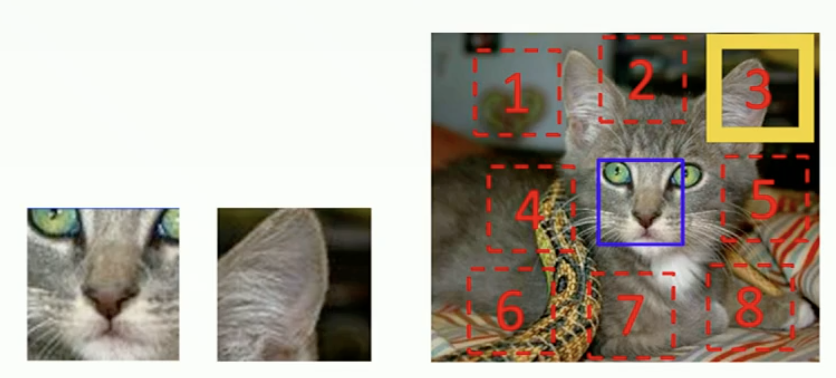
\includegraphics[scale=0.6]{images/spatial_context.png}
\end{center}
\subsubsection{Predicting Rotations(2018)}
\begin{center}
\includegraphics[scale=0.6]{images/predict-rotation.png}
\end{center}
\subsection{Contrastive Learning}
\begin{itemize}
\item Contrastive Learning: learned representations hsould be close together for similar inputs and far apart for dissimilar inputs.
\item If we have representation $z$ generated from some input $z$ with representations $z_1, \dots, z_k$ from other inputs.  
\begin{itemize}
\item If one of $z_1, \dots, z_k$ is generated from a similar input $z_+$, we have the most common contrastive learning loss 
$$- \log \frac{\exp(z^Tz_+ / \tau)}{\sum_{i=1}^K \exp(z^Tz_i/\tau)}.$$
\end{itemize}
\end{itemize}
\subsubsection{Contrastive Predictive Coding(CPC)(2018)}
\begin{itemize}
\item CPC defines similar as coming from the same input, which requires splitting up the input into multiple parts, and dissimilar as coming from different inputs.
\item This has been applied to audio, images, text.
\item Extracting a single representation from the whole input requires more work.
\end{itemize}
\begin{center}
\includegraphics[scale=0.4]{images/CPC.png}
\end{center}
\subsection{Data Augmentation}
\begin{itemize}
\item Many other types of data augmentations, besides rotations, can be leveraged to produce useful self-supervised learning signals in CV.  
\item However, instead of trying to predict the augmentation, we can use the augmentations in conjunction with contrastive learning.
\item Specifically, we consider different augmentations of the same image as similar and different images as dissimilar. 
\item Now we can learn representations of entire images directly, since we don't need to split up the image direction.
\end{itemize}
\subsubsection{Momentum Contrast(MoCo)(2019)}
\begin{itemize}
\item A key challenge in constrastive learning is sampling a sufficiently large and diverse set of dissimilar examples for training
\item If it is too large, then generating representations for all negatives will be expensive.
\item MoCo maintains a queue of negatives and adds it to every training iterations with the representations from the latest minibatch, pushing out the oldest minipatch.  
\item The small problem is that the representations at the end of the queue are not from the same model anymore.
\item Since the representation itself is changing, MoCo uses an exponential moving average(EMA) of the model parameters to generate representations for the queue, encouraging some similarity across mini batches.  
\end{itemize}
\subsubsection{SimCLR}
\begin{itemize}
\item We can remove the need for a queue if we incorporate larger batch sizes, longer training, larger models, stronger augmentations, and a few technical improvements.
\item These are summarized by SimCLR.  
\end{itemize}
 \begin{center}
\includegraphics[scale=0.6]{images/simclr.png}
\end{center}
\subsection{Bootstrap your own latent(BYOL)(2020)}
\begin{itemize}
\item Contrastive learning is popular, but there are other approaches.
\item One idea is to train two networks(the online and target or student and teacher).
\item in BYOL, the online and target are given two augmentations of the same input, and the online is optimized to try to predict the target's network representation.
\item The target network is updated as an EMA of the online network.
\end{itemize}
\subsection{Self-distillation with no labels (DINO)(2021)}
\begin{itemize}
\item Have the student try to match the probability values of the teacher.
\item They both get inputs and the teacher products some probability values and the student is trying to match these values. 
\item The idea is called \textbf{distillation} in the case where the teacher knows something; it has been pretrained on some dataset. 
\item Self-distillation is the self-supervised version of this, where it works well even when the teacher knows nothing.
\item The student is optimized to try to match the probability values and the teacher is updated with an EMA on the student parameters. 
\end{itemize}
\subsection{Multimodal Constrastive Learning: CLIP(2021)}
\begin{itemize}
\item We are increasingly seeing powerful multimodel models which combine information across modalities.
\item Contrastive language-image pretraining(CLIP) is one model trained on a large dataset of (image, text) pairs collected from the internet.  This is unlabeled data
\item The CLIP model has a text encoder and an image encoder where we output representations which we embed into the same embedding space with the same dimension so we can compare them directtly.  Then, we train with a contrastive objective where the (image, text) pairs are similar and all other non-pairs are dissimilar.
\item This is an important piece of the DALL.E 2 system. 
\end{itemize}
\pagebreak
\section{04/13/2022 - Massive Models}
We have models with over 100B parameters, and all of them are transformer decoder language models.  A natural question is to consider the scaling laws theoretically.  
\subsection{Scaling Laws}
\subsubsection{Scaling Laws for NLMs(2020)}
 \begin{center}
\includegraphics[scale=0.5]{images/kaplan.png}
\end{center}
Some weird things from these plots on the right:
\begin{itemize}
\item The scaling laws hold for over six orders of magnitude for the amount of available compute and model size.
\item Model size and dataset size need to be scaled together, but not equally : 8x model size requires only 5x dataset size.  This is disputed today by other work saying that equal scaling is best.
\item Larger models require fewer data points and optimization steps to reach the same performance as smaller models.
\item For a fixed compute budget, the best performance comes from training large models and stopping well short of convergence.
\end{itemize}

\subsubsection{Scaling Laws for autoregressive generative modeling(2020)}
\begin{center}
\includegraphics[scale=0.6]{images/henighan.png}
\end{center}
\subsection{Massive Models}
\subsubsection{GPT-3(2020)}
175B parameters, combined training set has 500B tokens.  The model never sees the whole dataset(only 300B).
\begin{center}
\includegraphics[scale=0.5]{images/gpt.png}
\end{center}
Some options we have are
\begin{itemize}
\item Zero shot: predict the answer only given a natural language description of the task . No gradient updates are performed
\item One-shot: in addition to the task description, the model sees a sinlge example of the task.  No gradient updates performed.
\item Few shot: in addition to the task description, the model sees a few examples of the task.  No gradient updates performed.
\end{itemize}
GPT-3 is very good at Few-shot learning, but there is significant room for improvement.
\subsubsection{Gopher(2021)}
\begin{itemize}
\item Gopher is a 280B parameter transformer decoder
\item 2T tokens but only trained for 300B tokens.
\item many different sizes of the model, architecture considered and huge dataset collected.  
\item applicable to a diverse set of NLP tasks. 
\end{itemize}
\subsubsection{Chinchilla(2022)}
\begin{itemize}
\item Chinchilla considers varying hyperparameters (primarily, learning rate schedule) that Kaplan et al held fixed, which leads to different scaling conclusions
\item They concluded that model and dataset size should scale \textbf{equally}
\item Tested on MAssive Multitask Language Understand(MMLU) which consists of exam questions from 57 academic subjects from elementary to professional level.
\end{itemize}
\subsubsection{Megatron-Turing NLG(2022)}
\begin{itemize}
\item MT-NLG is a 530B parameter transformer decoder
\item Training set is (a puny) 339B tokens, training is done with 270B tokens
\end{itemize}
\subsubsection{PaLM(2022)}
\begin{itemize}
\item PaLM is a 540B parameter (yes, you guessed it) transformer decoder
\item Training set: 780B tokens; training: one full epoch!
\end{itemize}
\subsection{Applications of Massive Models}
\subsubsection{Few-shot learning via Prompting}
\begin{itemize}
\item Provide some examples of the task within the model input itself
\item Prompt engineering is getting the model to perform the best by giving the best prompt
\item PaLM using chain-of-thought prompting which not only prompts the correct answer but also the process at which the answer is reached.  
\item Self-consistency(sampling multiple answers and picking the most consistent answer).
\end{itemize}
\subsubsection{Medium-shot learning with fine tuning}
\begin{itemize}
\item fine tuning refers to updating the model via gradient based optimization with a small data set.
\item This is usually not feasible with the large size of the models.
\item GPT-3 now offers fine tuning as part of the API.
\item When possible, fine tuning significantly outperforms prompting. 
\end{itemize}
\subsubsection{Specializing to Code: Codex and AlphaCode}
\begin{itemize}
\item Codex is a 12B parameter model and fine tunes on 159GB from GitHub.  This powers GitHub Copilot.
\item AlphaCode scales up to competition level coding, comparable to the median competitor.
\item 41B model size and 517B dataset size, model architecture is encoder-decoder, fine tuning on competition code, sampling/filtering many candidate solutions help in scaling to this level.
\end{itemize}
\subsection{Limitations of Massive Models}
\subsubsection{Challenge Tasks}
\begin{itemize}
\item Stress tests like ANLI significant room for improvement and scaling up doesn't solve this problem.
\item Hard tasks like solutions for high school math contests have low accuracy.
\item These models are trained/fine tuned with more text/code/math than a human will ever see, so it seems like something is missing. 
\end{itemize}
\subsubsection{Potential Harms and Biases}
\begin{itemize}
\item Papers come with a model card describing details, intended uses, and some analysis about potential harms. 
\item GPT-3 was analyzed for gender, race, and religion biases, and this shed light on its predispositions that seem in line with training. 
\item Analysis on Gopher (and, to an extent, PaLM) demonstrates that large models, when given a toxic prompt, are more likely to generate toxic continuations
\item 
\end{itemize}
\pagebreak
\section{04/18/2022 - Chelsea Finn: Meta Learning}
\begin{itemize}
\item Adapting to new objects
\item Adapting to new molecules
\item Adapting from simulation to real
\item Adapting to new regions of the world
\end{itemize}
\subsection{How does Meta-Learning Work?}
\begin{itemize}
\item Given 1 example of $5$ classes and some test sets, it would not be able to train on its own. 
\item Assume that we have other image data, split it into mini train sets and test sets. 
\item Hope that after doing the meta-training, we can meta-test with new classes.
\item Image classification can be replaced with regression, language generatioon, skill learning, or really any ML problem.
\end{itemize}
\begin{center}
\includegraphics[scale=0.6]{images/metatrain.png}
\end{center}
\subsection{Mathematical Formulation of Meta Learning}
In supervised learning, we have inputs $x$, outputs $y = g_\phi(x)$ and a dataset $\{(x, y)_i\}$.

In meta supervised learning, we have inputs $\mc D^{tr} = \{(x, y)_{1 : K}\}$ and $x^{ts}$, and the goal is to predict the corresponding label output $y^{ts} = f_\theta(\mc D^{tr}, x^{ts})$.  Now, we have a dataset of datasets $\{\mc D_i\}$, $\mc D_i = \{(x, y)_j\}$.

We reduce meta-learning to designing and optimizing $f$, which we can do using the dataset of datasets and end-to-end learning.
\subsection{Meta Learning Problem}
Given data from $\mc T_1, \dots, \mc T_n$, so a new task $\mc T_{test}.$ We have a key assumption: meta-training and meta-test task drawn i.i.d. from same task distribution.
$$\mc T_1, \dots, \mc T_n \sim p(\mc T), \mc T_j \sim p(\mc J).$$ 

The tasks can correspond to
\begin{itemize}
\item Recognizing handwritten digits from new languages
\item Giving feedback to students on different exams
\item classifying species in different regions of the world
\item a robot performing different tasks
\end{itemize}
In general, the more tasks, the better.

\subsubsection{Other Similar Problems}
\begin{itemize}
\item \textbf{Multi-Task Learning}: solve multiple tasks $\mc T_1, \dots, \mc T_T$ at once:
$$\min_\theta \sum_{i=1}^T \mc L_i(\theta, \mc D_i).$$
\item \textbf{Transfer Learning}: Solve target task $\mc T_b$ after solving source task $\mc T_a$ by transferring knowledge from $\mc T_a$.
\item \textbf{Meta-Learning}: Given data from $\mc T_1, \dots, \mc T_n$ solve $\mc T_{test}$.
\end{itemize}
In Meta-Learning and Transfer Learning, we generally assume we don't have access to prior tasks, but in all of these settings the tasks all share some prior structure. 

\subsubsection{Terminology}
\begin{itemize}
\item $D_i^{tr}$: support set
\item $D_i^{test}$: query set
\item k-shot learning: learning with $k$ exmaples per class
\item $N$-way classification: choosing between N different classes. 
\end{itemize}
\begin{center}
\includegraphics[scale=0.6]{images/metaterm.png}
\end{center}
\subsubsection{Black-Box Meta-Learning}
\begin{center}
\includegraphics[scale=0.6]{images/blackmeta.png}
\end{center}
The first key idea is to parameterize the learner as a neural network.  This is expressive but it is a challenging optimization problem. 
\begin{center}
\includegraphics[scale=0.6]{images/gradmeta.png}
\end{center}
The next key is to embed gradient descent into this, which embeds optimizing inside the learning process.   This can mostly be handled by PyTorch/TensorFlow. This gives us the structure of optimization embedded into the meta leraning, but requires a second-order optimization.

\subsubsection{General Few Shot Meta-Learning Algorithm}:
For meta-training:
\begin{enumerate}
\item Sample task $T_i$
\item Sample disjoint datasets $D_i^{tr}, D_i^{test}$ from $D_i$.
\item Compute $\phi_i \leftarrow f_\theta(D_i^{tr})$
\item Update $\theta$ using $\nabla_\theta \mc L(\phi_i, \mc D_i^{test})$.
\end{enumerate}
For meta-testing:
\begin{enumerate}
\item Given train set $D_j^{tr}$ for new task $T_j$
\item Compute $\phi_j \leftarrow f_\theta(D_j^{tr})$.
\end{enumerate}
\subsection{Non-Parametric Few-Shot Learning}
Non-parametric methods like k-nn are simple for low data regimes, and they work reasonably well.  During meta-test time, we are in the low data regime, but in meta-training we want to be parametric since we have a large amount of data. So the goal is to use parametric meta-learners to produce effective non-parametric learners.
\subsubsection{Non-parametric Methods}
First, using nearest neighbors from the test data points and find the nearest training example.  Then, output the corresponding label.  What distance do we use? $\ell_2$ distance in pixel space is not very good.  Instead, we will use the meta-training data to predict whether two networks are similar:  
\begin{center}
\includegraphics[scale=0.6]{images/twin.png}
\end{center}
This is similar to BYOL.  Then, in test time we we compare the image $x_{test}$ to each image in $D_j^{tr}$.  Then, meta-training is binary classification and meta-test is N-way classification.  Can we match them? We can do this by checking similarity in a learned embedding space via nearest neighbors.
\begin{center}
\includegraphics[scale=0.3]{images/embedmeta.png}
\end{center}
\subsubsection{Algorithm}
\begin{enumerate}
\item Sample task $T_i$
\item Sample disjoint datasets $D_i^{tr}, D_i^{test}$ from $D_i$
\item Compute $\hat{y}^{ts} = \sum_{x_k, y_k \in D^{tr}} f_\theta(x^{ts}, x_k), y_k$.
\item Update $\theta$ using $\nabla_\theta L(\hat{y^{ts}}, y^{ts})$.
\end{enumerate}
What if we have $>1$ shot? Matching networks will do the comparisons independently.  Can we aggregate the class information into a prototypical embedding?
\subsubsection{Prototypical Networks}
Average samples of each class into a prototype, embed $x$ into the embedded space and perform NN in the embedding space using the prototypes.
\begin{center}
\includegraphics[scale=0.6]{images/proto.png}
\end{center}

Other approaches:
\begin{itemize}
\item Learn non-linear relation module on embeddings
\item Learn infinite mixture of prototypes
\item Perform message passing on embeddings using Graph Neural Networks.
\end{itemize}
\subsection{Case Study: Feedback Generation}
Train a model to give feedback on an open-ended python code snippet. Infer student misconceptions $y$ from student solution $x$.

Why this is difficult?
\begin{itemize}
\item Limited annotations: grading student work tasks expert knowledge and is time consuming. 
\item Long-tailed distribution: students can solve the same problem in many ways.
\item Changing curriculums: instructors constantly edit problems and solutions.
\end{itemize}

\subsubsection{Framing as Meta-Learning}
\begin{itemize}
\item Training Dataset: 4 final exams and 4 midterm exams with a rubric
\item We can set each item on the rubric as a task. 
\end{itemize}
\subsection{ProtoTransformer}
\begin{center}
\includegraphics[scale=0.3]{images/prototrans.png}
\end{center}
This doesn't work out of the box what some tricks are:
\begin{itemize}
\item Augment rubric tasks with self-supervised tasks
\item Reduce few-shot ambiguity by incorporating side information
\item Pre-train on unlabled Python code.
\end{itemize}
\subsection{Overview of Meta-Learners}
\begin{center}
\includegraphics[scale=0.3]{images/prop1.png}
\end{center}\begin{center}
\includegraphics[scale=0.3]{images/prop2.png}
\end{center}\begin{center}
\includegraphics[scale=0.3]{images/prop3.png}
\end{center}
\pagebreak
\section{04/20/2022 - Sergey Levine: Deep Reinforcement Learning} 
\subsection{From Prediction to Control: Challenges}
\begin{itemize}
\item In prediction, we assume the data is i.i.d., so $p(D) = \prod_i p(y_i | x_i) p(x_i)$.  But in control, the choices you make earlier can influence the change you make later.  For example, making a turn on a curved road. The iid assumption focus on getting the highest overall average accuracy which may not be ideal.
\item In supervised learning you have a ground truth label, in control you have a goal.
\item In supervised learning, you want to predict the right label, in control you want to accomplish the task.
\end{itemize}
These are not just issues for control, we have the same feedback issues in real-world deployment of ML. 
\subsection{Terminology}
Input: $o_t$ for observation, output $a_t$ for action.  Policy $\pi_\theta(a_t | o_t)$. We also have states $s_t$.  The difference between states and observation is that the state is the sufficient information to fully describe the system right now, so that we don't need to know anything about the past to predict the future.  The observation is like the image with all the pixels and we can't necessarily use the observation on it's own to figure out future without previous images. 
 \begin{center}
\includegraphics[scale=0.6]{images/bayes.png}
\end{center}
We have the markov property, which gives that the future is independent of the past at each state.  
\subsection{Imitation Learning}
\subsubsection{Behavioral Cloning}
Example: driving an autonomous vehicle.  The observations are images from dashboard camera and actions are steering commands.

We use data from human drivers giving pairs $(o_t, a_t)$ giving training data.  Then, let's just do supervised learning and map images to steering commands!

This is called \textbf{behavioral cloning}.

\begin{itemize}
\item The theoretician would say this does not work.  When you move off the support of the data, it will make mistakes and compound:
\begin{center}
\includegraphics[scale=0.3]{images/cloning.png}
\end{center}

\item In the real world, it works pretty well? NVIDIA Research initially said no but after some 3000 miles of training, it works!
\end{itemize}
Why does it work?  The main issue is distribution shift: $p_{data}(o_t) \ne p_{\pi_\theta}(o_t)$.  What did they do to make it work?  A data augmentation trick where they have a right and left camera from training that is biased to stay centered.
\subsubsection{DAgger: Dataset Aggregation}
Can we make $p_{data}(o_t) = p_{\pi_{\theta}}(o_t)$ in general? Instead of being clever about $p_{\pi_\theta}(o_t)$, be clever about $p_{data}(o_t)$.

The goal: collect training data from $p_{\pi_theta}(o_t)$ instead of $p_{data}(o_t)$.  Run $\pi_\theta(a_t| o_t)$ and ask humans to label them.
\begin{enumerate}
\item train $\pi_theta(a_t|o_t)$ from human data $D = \{o_1, a_1, \dots, o_n, a_n\}$.
\item run $\pi_\theta(a_t | o_t)$ to get dataset $D_\pi = \{o_1, \dots, o_m\}$
\item ask human to label $D_\pi$ with actions $a_t$
\item aggregate $D \leftarrow D \cup D_\pi$.
\end{enumerate}
The problems with this are that it requires costly data collection and labeling. 
\subsection{Q-Learning}
\begin{center}
\includegraphics[scale=0.3]{images/qlearn.png}
\end{center}
Off-policy Q-learning:
\begin{enumerate}
\item Collect data $\{s_i, a_i, s_i', r_i\}$ using some policy, add it to $B$.
\item Sample a batch $(s_i, a_i, s_i', r_i)$ from $B$
\item Minimize $\sum_i (Q(s_i, a_i) - [r(s_i, a_i) + \max_{a_i'}Q(s_i', a_i')])^2$
\item Go to step 2 and repeat as many times as wanted.
\end{enumerate}
\subsection{Offline RL}
We want data-driven RL methods.  There is a large gulf between problems that are solved well via RL and problems solved via deep learning. 
\begin{center}
\includegraphics[scale=0.4]{images/offline.png}
\end{center}
\subsubsection{Offline RL Workflow}
\begin{enumerate}
\item Collect a dataset using any policy or mixture of policies
\item Run offline RL on the dataset to learn a policy
\item Deploy in the real world, and retrain until we have the model we want.
\end{enumerate}
The problem?
How well it does is much worse than it thinks it does because of distribution shift. 
\subsubsection{Conservative Q}
Big Q-values are troublesome.  So we penalize these:
\begin{center}
\includegraphics[scale=0.4]{images/consq.png}
\end{center}
\begin{center}
\includegraphics[scale=0.4]{images/consq2.png}
\end{center}
\end{document}

